% Options for packages loaded elsewhere
% Options for packages loaded elsewhere
\PassOptionsToPackage{unicode}{hyperref}
\PassOptionsToPackage{hyphens}{url}
\PassOptionsToPackage{dvipsnames,svgnames,x11names}{xcolor}
%
\documentclass[
]{article}
\usepackage{xcolor}
\usepackage{amsmath,amssymb}
\setcounter{secnumdepth}{5}
\usepackage{iftex}
\ifPDFTeX
  \usepackage[T1]{fontenc}
  \usepackage[utf8]{inputenc}
  \usepackage{textcomp} % provide euro and other symbols
\else % if luatex or xetex
  \usepackage{unicode-math} % this also loads fontspec
  \defaultfontfeatures{Scale=MatchLowercase}
  \defaultfontfeatures[\rmfamily]{Ligatures=TeX,Scale=1}
\fi
\usepackage{lmodern}
\ifPDFTeX\else
  % xetex/luatex font selection
\fi
% Use upquote if available, for straight quotes in verbatim environments
\IfFileExists{upquote.sty}{\usepackage{upquote}}{}
\IfFileExists{microtype.sty}{% use microtype if available
  \usepackage[]{microtype}
  \UseMicrotypeSet[protrusion]{basicmath} % disable protrusion for tt fonts
}{}
\makeatletter
\@ifundefined{KOMAClassName}{% if non-KOMA class
  \IfFileExists{parskip.sty}{%
    \usepackage{parskip}
  }{% else
    \setlength{\parindent}{0pt}
    \setlength{\parskip}{6pt plus 2pt minus 1pt}}
}{% if KOMA class
  \KOMAoptions{parskip=half}}
\makeatother
% Make \paragraph and \subparagraph free-standing
\makeatletter
\ifx\paragraph\undefined\else
  \let\oldparagraph\paragraph
  \renewcommand{\paragraph}{
    \@ifstar
      \xxxParagraphStar
      \xxxParagraphNoStar
  }
  \newcommand{\xxxParagraphStar}[1]{\oldparagraph*{#1}\mbox{}}
  \newcommand{\xxxParagraphNoStar}[1]{\oldparagraph{#1}\mbox{}}
\fi
\ifx\subparagraph\undefined\else
  \let\oldsubparagraph\subparagraph
  \renewcommand{\subparagraph}{
    \@ifstar
      \xxxSubParagraphStar
      \xxxSubParagraphNoStar
  }
  \newcommand{\xxxSubParagraphStar}[1]{\oldsubparagraph*{#1}\mbox{}}
  \newcommand{\xxxSubParagraphNoStar}[1]{\oldsubparagraph{#1}\mbox{}}
\fi
\makeatother

\usepackage{color}
\usepackage{fancyvrb}
\newcommand{\VerbBar}{|}
\newcommand{\VERB}{\Verb[commandchars=\\\{\}]}
\DefineVerbatimEnvironment{Highlighting}{Verbatim}{commandchars=\\\{\}}
% Add ',fontsize=\small' for more characters per line
\usepackage{framed}
\definecolor{shadecolor}{RGB}{241,243,245}
\newenvironment{Shaded}{\begin{snugshade}}{\end{snugshade}}
\newcommand{\AlertTok}[1]{\textcolor[rgb]{0.68,0.00,0.00}{#1}}
\newcommand{\AnnotationTok}[1]{\textcolor[rgb]{0.37,0.37,0.37}{#1}}
\newcommand{\AttributeTok}[1]{\textcolor[rgb]{0.40,0.45,0.13}{#1}}
\newcommand{\BaseNTok}[1]{\textcolor[rgb]{0.68,0.00,0.00}{#1}}
\newcommand{\BuiltInTok}[1]{\textcolor[rgb]{0.00,0.23,0.31}{#1}}
\newcommand{\CharTok}[1]{\textcolor[rgb]{0.13,0.47,0.30}{#1}}
\newcommand{\CommentTok}[1]{\textcolor[rgb]{0.37,0.37,0.37}{#1}}
\newcommand{\CommentVarTok}[1]{\textcolor[rgb]{0.37,0.37,0.37}{\textit{#1}}}
\newcommand{\ConstantTok}[1]{\textcolor[rgb]{0.56,0.35,0.01}{#1}}
\newcommand{\ControlFlowTok}[1]{\textcolor[rgb]{0.00,0.23,0.31}{\textbf{#1}}}
\newcommand{\DataTypeTok}[1]{\textcolor[rgb]{0.68,0.00,0.00}{#1}}
\newcommand{\DecValTok}[1]{\textcolor[rgb]{0.68,0.00,0.00}{#1}}
\newcommand{\DocumentationTok}[1]{\textcolor[rgb]{0.37,0.37,0.37}{\textit{#1}}}
\newcommand{\ErrorTok}[1]{\textcolor[rgb]{0.68,0.00,0.00}{#1}}
\newcommand{\ExtensionTok}[1]{\textcolor[rgb]{0.00,0.23,0.31}{#1}}
\newcommand{\FloatTok}[1]{\textcolor[rgb]{0.68,0.00,0.00}{#1}}
\newcommand{\FunctionTok}[1]{\textcolor[rgb]{0.28,0.35,0.67}{#1}}
\newcommand{\ImportTok}[1]{\textcolor[rgb]{0.00,0.46,0.62}{#1}}
\newcommand{\InformationTok}[1]{\textcolor[rgb]{0.37,0.37,0.37}{#1}}
\newcommand{\KeywordTok}[1]{\textcolor[rgb]{0.00,0.23,0.31}{\textbf{#1}}}
\newcommand{\NormalTok}[1]{\textcolor[rgb]{0.00,0.23,0.31}{#1}}
\newcommand{\OperatorTok}[1]{\textcolor[rgb]{0.37,0.37,0.37}{#1}}
\newcommand{\OtherTok}[1]{\textcolor[rgb]{0.00,0.23,0.31}{#1}}
\newcommand{\PreprocessorTok}[1]{\textcolor[rgb]{0.68,0.00,0.00}{#1}}
\newcommand{\RegionMarkerTok}[1]{\textcolor[rgb]{0.00,0.23,0.31}{#1}}
\newcommand{\SpecialCharTok}[1]{\textcolor[rgb]{0.37,0.37,0.37}{#1}}
\newcommand{\SpecialStringTok}[1]{\textcolor[rgb]{0.13,0.47,0.30}{#1}}
\newcommand{\StringTok}[1]{\textcolor[rgb]{0.13,0.47,0.30}{#1}}
\newcommand{\VariableTok}[1]{\textcolor[rgb]{0.07,0.07,0.07}{#1}}
\newcommand{\VerbatimStringTok}[1]{\textcolor[rgb]{0.13,0.47,0.30}{#1}}
\newcommand{\WarningTok}[1]{\textcolor[rgb]{0.37,0.37,0.37}{\textit{#1}}}

\usepackage{longtable,booktabs,array}
\usepackage{calc} % for calculating minipage widths
% Correct order of tables after \paragraph or \subparagraph
\usepackage{etoolbox}
\makeatletter
\patchcmd\longtable{\par}{\if@noskipsec\mbox{}\fi\par}{}{}
\makeatother
% Allow footnotes in longtable head/foot
\IfFileExists{footnotehyper.sty}{\usepackage{footnotehyper}}{\usepackage{footnote}}
\makesavenoteenv{longtable}
\usepackage{graphicx}
\makeatletter
\newsavebox\pandoc@box
\newcommand*\pandocbounded[1]{% scales image to fit in text height/width
  \sbox\pandoc@box{#1}%
  \Gscale@div\@tempa{\textheight}{\dimexpr\ht\pandoc@box+\dp\pandoc@box\relax}%
  \Gscale@div\@tempb{\linewidth}{\wd\pandoc@box}%
  \ifdim\@tempb\p@<\@tempa\p@\let\@tempa\@tempb\fi% select the smaller of both
  \ifdim\@tempa\p@<\p@\scalebox{\@tempa}{\usebox\pandoc@box}%
  \else\usebox{\pandoc@box}%
  \fi%
}
% Set default figure placement to htbp
\def\fps@figure{htbp}
\makeatother


% definitions for citeproc citations
\NewDocumentCommand\citeproctext{}{}
\NewDocumentCommand\citeproc{mm}{%
  \begingroup\def\citeproctext{#2}\cite{#1}\endgroup}
\makeatletter
 % allow citations to break across lines
 \let\@cite@ofmt\@firstofone
 % avoid brackets around text for \cite:
 \def\@biblabel#1{}
 \def\@cite#1#2{{#1\if@tempswa , #2\fi}}
\makeatother
\newlength{\cslhangindent}
\setlength{\cslhangindent}{1.5em}
\newlength{\csllabelwidth}
\setlength{\csllabelwidth}{3em}
\newenvironment{CSLReferences}[2] % #1 hanging-indent, #2 entry-spacing
 {\begin{list}{}{%
  \setlength{\itemindent}{0pt}
  \setlength{\leftmargin}{0pt}
  \setlength{\parsep}{0pt}
  % turn on hanging indent if param 1 is 1
  \ifodd #1
   \setlength{\leftmargin}{\cslhangindent}
   \setlength{\itemindent}{-1\cslhangindent}
  \fi
  % set entry spacing
  \setlength{\itemsep}{#2\baselineskip}}}
 {\end{list}}
\usepackage{calc}
\newcommand{\CSLBlock}[1]{\hfill\break\parbox[t]{\linewidth}{\strut\ignorespaces#1\strut}}
\newcommand{\CSLLeftMargin}[1]{\parbox[t]{\csllabelwidth}{\strut#1\strut}}
\newcommand{\CSLRightInline}[1]{\parbox[t]{\linewidth - \csllabelwidth}{\strut#1\strut}}
\newcommand{\CSLIndent}[1]{\hspace{\cslhangindent}#1}



\setlength{\emergencystretch}{3em} % prevent overfull lines

\providecommand{\tightlist}{%
  \setlength{\itemsep}{0pt}\setlength{\parskip}{0pt}}



 


\makeatletter
\@ifpackageloaded{tcolorbox}{}{\usepackage[skins,breakable]{tcolorbox}}
\@ifpackageloaded{fontawesome5}{}{\usepackage{fontawesome5}}
\definecolor{quarto-callout-color}{HTML}{909090}
\definecolor{quarto-callout-note-color}{HTML}{0758E5}
\definecolor{quarto-callout-important-color}{HTML}{CC1914}
\definecolor{quarto-callout-warning-color}{HTML}{EB9113}
\definecolor{quarto-callout-tip-color}{HTML}{00A047}
\definecolor{quarto-callout-caution-color}{HTML}{FC5300}
\definecolor{quarto-callout-color-frame}{HTML}{acacac}
\definecolor{quarto-callout-note-color-frame}{HTML}{4582ec}
\definecolor{quarto-callout-important-color-frame}{HTML}{d9534f}
\definecolor{quarto-callout-warning-color-frame}{HTML}{f0ad4e}
\definecolor{quarto-callout-tip-color-frame}{HTML}{02b875}
\definecolor{quarto-callout-caution-color-frame}{HTML}{fd7e14}
\makeatother
\makeatletter
\@ifpackageloaded{caption}{}{\usepackage{caption}}
\AtBeginDocument{%
\ifdefined\contentsname
  \renewcommand*\contentsname{Table of contents}
\else
  \newcommand\contentsname{Table of contents}
\fi
\ifdefined\listfigurename
  \renewcommand*\listfigurename{List of Figures}
\else
  \newcommand\listfigurename{List of Figures}
\fi
\ifdefined\listtablename
  \renewcommand*\listtablename{List of Tables}
\else
  \newcommand\listtablename{List of Tables}
\fi
\ifdefined\figurename
  \renewcommand*\figurename{Figure}
\else
  \newcommand\figurename{Figure}
\fi
\ifdefined\tablename
  \renewcommand*\tablename{Table}
\else
  \newcommand\tablename{Table}
\fi
}
\@ifpackageloaded{float}{}{\usepackage{float}}
\floatstyle{ruled}
\@ifundefined{c@chapter}{\newfloat{codelisting}{h}{lop}}{\newfloat{codelisting}{h}{lop}[chapter]}
\floatname{codelisting}{Listing}
\newcommand*\listoflistings{\listof{codelisting}{List of Listings}}
\makeatother
\makeatletter
\makeatother
\makeatletter
\@ifpackageloaded{caption}{}{\usepackage{caption}}
\@ifpackageloaded{subcaption}{}{\usepackage{subcaption}}
\makeatother
\usepackage{bookmark}
\IfFileExists{xurl.sty}{\usepackage{xurl}}{} % add URL line breaks if available
\urlstyle{same}
\hypersetup{
  pdftitle={Análisis de Supervivencia},
  pdfauthor={Sergio M. Nava Muñoz},
  colorlinks=true,
  linkcolor={blue},
  filecolor={Maroon},
  citecolor={Blue},
  urlcolor={Blue},
  pdfcreator={LaTeX via pandoc}}


\title{Análisis de Supervivencia}
\usepackage{etoolbox}
\makeatletter
\providecommand{\subtitle}[1]{% add subtitle to \maketitle
  \apptocmd{\@title}{\par {\large #1 \par}}{}{}
}
\makeatother
\subtitle{Estimación no paramétrica}
\author{Sergio M. Nava Muñoz}
\date{2025-06-01}
\begin{document}
\maketitle

\renewcommand*\contentsname{Table of contents}
{
\hypersetup{linkcolor=}
\setcounter{tocdepth}{2}
\tableofcontents
}

\section{Estimación no
paramétrica}\label{estimaciuxf3n-no-paramuxe9trica}

\subsection{Temario de la Sesión}\label{temario-de-la-sesiuxf3n}

\begin{itemize}
\item
  \textbf{Fundamentos:} ¿Qué es el análisis de supervivencia y cómo se
  estructuran los datos (tiempo, evento y censura)?
\item
  \textbf{El Estimador Kaplan-Meier:} Introducción al método no
  paramétrico fundamental para estimar la función de supervivencia
  cuando hay datos censurados.
\item
  \textbf{Cálculo e Interpretación:} Un ejemplo paso a paso para
  calcular e interpretar una curva de Kaplan-Meier.
\item
  \textbf{Comparación entre Grupos:} Uso de la prueba Log-Rank para
  determinar si existen diferencias significativas entre las curvas de
  supervivencia.
\item
  \textbf{Aplicación Práctica en R:} Implementación de estas técnicas
  utilizando paquetes como \texttt{survival} y \texttt{survminer}.
\end{itemize}

\subsection{La función de distribución acumulada empírica
(FDAE)}\label{la-funciuxf3n-de-distribuciuxf3n-acumulada-empuxedrica-fdae}

Dada una muestra de tiempos de falla sin censura:

\[
\hat{F}(t) = \frac{\#\{T_i \leq t\}}{n}
\]

Es un estimador escalonado, que da saltos en cada observación.\\
La función de supervivencia empírica se define como:

\[
\hat{S}(t) = 1 - \hat{F}(t)
\]

\textbf{Limitación}: no puede manejar adecuadamente datos censurados.

\pandocbounded{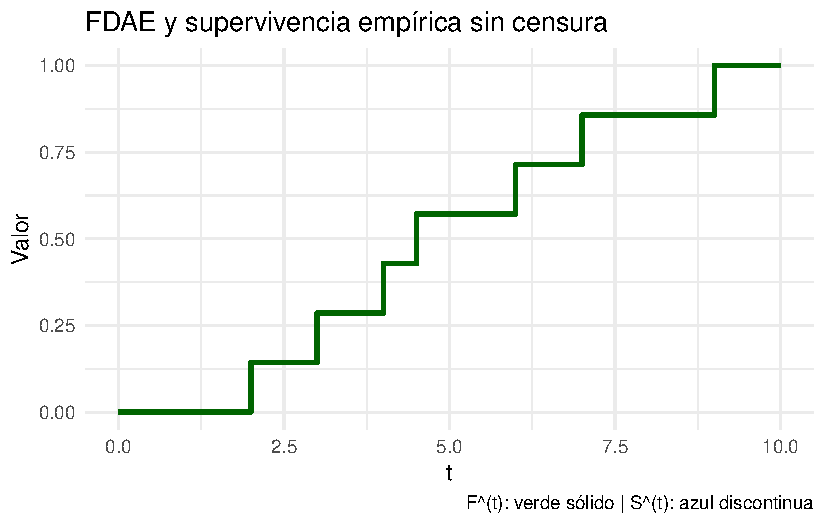
\includegraphics[keepaspectratio]{Unidad3_files/figure-pdf/unnamed-chunk-2-1.pdf}}

\pandocbounded{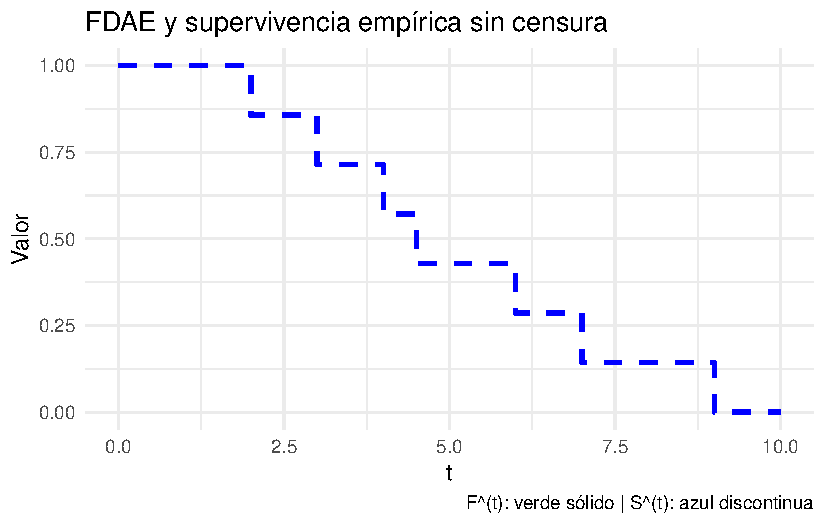
\includegraphics[keepaspectratio]{Unidad3_files/figure-pdf/unnamed-chunk-2-2.pdf}}

\begin{center}\rule{0.5\linewidth}{0.5pt}\end{center}

\subsection{Ejemplo en R: FDAE}\label{ejemplo-en-r-fdae}

\begin{longtable}[]{@{}rrr@{}}
\toprule\noalign{}
t & F\_hat & S\_hat \\
\midrule\noalign{}
\endhead
\bottomrule\noalign{}
\endlastfoot
0.0 & 0.0000000 & 1.0000000 \\
2.0 & 0.1428571 & 0.8571429 \\
3.0 & 0.2857143 & 0.7142857 \\
4.0 & 0.4285714 & 0.5714286 \\
4.5 & 0.5714286 & 0.4285714 \\
6.0 & 0.7142857 & 0.2857143 \\
7.0 & 0.8571429 & 0.1428571 \\
9.0 & 1.0000000 & 0.0000000 \\
10.0 & 1.0000000 & 0.0000000 \\
\end{longtable}

\pandocbounded{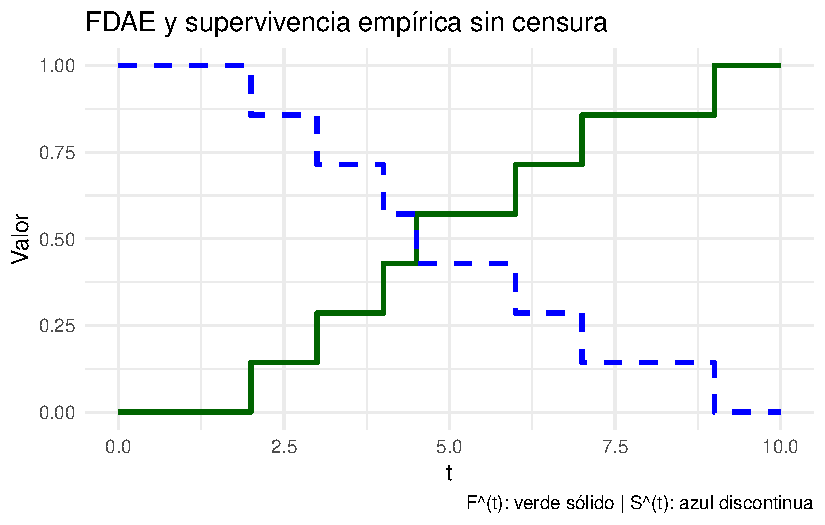
\includegraphics[keepaspectratio]{Unidad3_files/figure-pdf/unnamed-chunk-4-1.pdf}}

\begin{center}\rule{0.5\linewidth}{0.5pt}\end{center}

\subsection{Estimador de Kaplan-Meier}\label{estimador-de-kaplan-meier}

Cuando hay censura, la FDAE no es válida. Kaplan-Meier estima la función
de supervivencia como:

\[
\hat{S}(t) = \prod_{t_i \leq t} \left(1 - \frac{m_i}{n_i} \right)
\]

donde:

\begin{itemize}
\tightlist
\item
  \(m_i\): número de eventos en el tiempo \(t_i\)
\item
  \(n_i\): número de individuos en riesgo justo antes de \(t_i\)
\end{itemize}

Es un estimador escalonado que \textbf{ajusta el denominador} cuando hay
censura.

\begin{tcolorbox}[enhanced jigsaw, rightrule=.15mm, toprule=.15mm, colback=white, bottomrule=.15mm, bottomtitle=1mm, left=2mm, leftrule=.75mm, arc=.35mm, breakable, title=\textcolor{quarto-callout-note-color}{\faInfo}\hspace{0.5em}{Ejemplo}, opacitybacktitle=0.6, colframe=quarto-callout-note-color-frame, opacityback=0, toptitle=1mm, coltitle=black, titlerule=0mm, colbacktitle=quarto-callout-note-color!10!white]

\begin{longtable}[]{@{}rrrrr@{}}
\caption{Comparación entre FDAE, Supervivencia Empírica y
Kaplan-Meier}\tabularnewline
\toprule\noalign{}
tiempo & status & FDAE & S\_empirica & Kaplan\_Meier \\
\midrule\noalign{}
\endfirsthead
\toprule\noalign{}
tiempo & status & FDAE & S\_empirica & Kaplan\_Meier \\
\midrule\noalign{}
\endhead
\bottomrule\noalign{}
\endlastfoot
2.0 & 1 & 0.1667 & 0.8333 & 0.8750 \\
3.0 & 1 & 0.3333 & 0.6667 & 0.7500 \\
4.0 & 1 & 0.5000 & 0.5000 & 0.6250 \\
4.5 & 0 & 0.5000 & 0.5000 & 0.6250 \\
6.0 & 1 & 0.6667 & 0.3333 & 0.4688 \\
7.0 & 1 & 0.8333 & 0.1667 & 0.3125 \\
9.0 & 0 & 0.8333 & 0.1667 & 0.3125 \\
10.0 & 1 & 1.0000 & 0.0000 & 0.0000 \\
\end{longtable}

\end{tcolorbox}

\section{Cálculo e interpretación de
KM}\label{cuxe1lculo-e-interpretaciuxf3n-de-km}

\subsection{Esquema General de Datos}\label{esquema-general-de-datos}

\begin{longtable}[]{@{}
  >{\raggedright\arraybackslash}p{(\linewidth - 12\tabcolsep) * \real{0.1692}}
  >{\raggedright\arraybackslash}p{(\linewidth - 12\tabcolsep) * \real{0.1385}}
  >{\raggedright\arraybackslash}p{(\linewidth - 12\tabcolsep) * \real{0.1385}}
  >{\raggedright\arraybackslash}p{(\linewidth - 12\tabcolsep) * \real{0.1385}}
  >{\raggedright\arraybackslash}p{(\linewidth - 12\tabcolsep) * \real{0.1385}}
  >{\raggedright\arraybackslash}p{(\linewidth - 12\tabcolsep) * \real{0.1385}}
  >{\raggedright\arraybackslash}p{(\linewidth - 12\tabcolsep) * \real{0.1385}}@{}}
\caption{Esquema General de Datos con Subíndices}\tabularnewline
\toprule\noalign{}
\begin{minipage}[b]{\linewidth}\raggedright
No.~Indiv.
\end{minipage} & \begin{minipage}[b]{\linewidth}\raggedright
\(t\)
\end{minipage} & \begin{minipage}[b]{\linewidth}\raggedright
\(D\)
\end{minipage} & \begin{minipage}[b]{\linewidth}\raggedright
\(X_1\)
\end{minipage} & \begin{minipage}[b]{\linewidth}\raggedright
\(X_2\)
\end{minipage} & \begin{minipage}[b]{\linewidth}\raggedright
\ldots{}
\end{minipage} & \begin{minipage}[b]{\linewidth}\raggedright
\(X_p\)
\end{minipage} \\
\midrule\noalign{}
\endfirsthead
\toprule\noalign{}
\begin{minipage}[b]{\linewidth}\raggedright
No.~Indiv.
\end{minipage} & \begin{minipage}[b]{\linewidth}\raggedright
\(t\)
\end{minipage} & \begin{minipage}[b]{\linewidth}\raggedright
\(D\)
\end{minipage} & \begin{minipage}[b]{\linewidth}\raggedright
\(X_1\)
\end{minipage} & \begin{minipage}[b]{\linewidth}\raggedright
\(X_2\)
\end{minipage} & \begin{minipage}[b]{\linewidth}\raggedright
\ldots{}
\end{minipage} & \begin{minipage}[b]{\linewidth}\raggedright
\(X_p\)
\end{minipage} \\
\midrule\noalign{}
\endhead
\bottomrule\noalign{}
\endlastfoot
1 & \(t_1\) & \(D_1\) & \(X_{11}\) & \(X_{12}\) & \(\cdots\) &
\(X_{1p}\) \\
2 & \(t_2\) & \(D_2\) & \(X_{21}\) & \(X_{22}\) & \(\cdots\) &
\(X_{2p}\) \\
\ldots{} & \(\cdots\) & \(\cdots\) & \(\cdots\) & \(\cdots\) &
\(\cdots\) & \(\cdots\) \\
\(n\) & \(t_n\) & \(D_n\) & \(X_{n1}\) & \(X_{n2}\) & \(\cdots\) &
\(X_{np}\) \\
\end{longtable}

\begin{longtable}[]{@{}
  >{\raggedright\arraybackslash}p{(\linewidth - 6\tabcolsep) * \real{0.2741}}
  >{\raggedright\arraybackslash}p{(\linewidth - 6\tabcolsep) * \real{0.1556}}
  >{\raggedright\arraybackslash}p{(\linewidth - 6\tabcolsep) * \real{0.3333}}
  >{\raggedright\arraybackslash}p{(\linewidth - 6\tabcolsep) * \real{0.2370}}@{}}
\caption{Disposición alternativa de los datos ordenados}\tabularnewline
\toprule\noalign{}
\begin{minipage}[b]{\linewidth}\raggedright
Tiempos de fallo ordenados \(t_{(f)}\)
\end{minipage} & \begin{minipage}[b]{\linewidth}\raggedright
Núm. de fallos \(m_f\)
\end{minipage} & \begin{minipage}[b]{\linewidth}\raggedright
Censurados en \([t_{(f)}, t_{(f+1)})\), \(q_f\)
\end{minipage} & \begin{minipage}[b]{\linewidth}\raggedright
Conjunto de riesgo \(R(t_{(f)})\)
\end{minipage} \\
\midrule\noalign{}
\endfirsthead
\toprule\noalign{}
\begin{minipage}[b]{\linewidth}\raggedright
Tiempos de fallo ordenados \(t_{(f)}\)
\end{minipage} & \begin{minipage}[b]{\linewidth}\raggedright
Núm. de fallos \(m_f\)
\end{minipage} & \begin{minipage}[b]{\linewidth}\raggedright
Censurados en \([t_{(f)}, t_{(f+1)})\), \(q_f\)
\end{minipage} & \begin{minipage}[b]{\linewidth}\raggedright
Conjunto de riesgo \(R(t_{(f)})\)
\end{minipage} \\
\midrule\noalign{}
\endhead
\bottomrule\noalign{}
\endlastfoot
\(t_{(0)}\) & \(m_0\) & \(q_0\) & \(R(t_{(0)})\) \\
\(t_{(1)}\) & \(m_1\) & \(q_1\) & \(R(t_{(1)})\) \\
\(t_{(2)}\) & \(m_2\) & \(q_2\) & \(R(t_{(2)})\) \\
\(\cdots\) & \(\cdots\) & \(\cdots\) & \(\cdots\) \\
\(t_{(k)}\) & \(m_k\) & \(q_k\) & \(R(t_{(k)})\) \\
\end{longtable}

\begin{tcolorbox}[enhanced jigsaw, rightrule=.15mm, toprule=.15mm, colback=white, bottomrule=.15mm, bottomtitle=1mm, left=2mm, leftrule=.75mm, arc=.35mm, breakable, title=\textcolor{quarto-callout-note-color}{\faInfo}\hspace{0.5em}{Disposición alternativa de los datos ordenados}, opacitybacktitle=0.6, colframe=quarto-callout-note-color-frame, opacityback=0, toptitle=1mm, coltitle=black, titlerule=0mm, colbacktitle=quarto-callout-note-color!10!white]

Una disposición alternativa de los datos se muestra a continuación.\\
Esta organización es la base sobre la cual se derivan las curvas de
supervivencia de Kaplan-Meier.

\begin{itemize}
\tightlist
\item
  La primera columna de la tabla presenta los tiempos de supervivencia
  ordenados de menor a mayor. \(t_{(f)}\)
\item
  La segunda columna muestra el conteo de fallos en cada uno de los
  tiempos de fallo distintos. \(m_{f}\)
\item
  La tercera columna presenta los conteos de censura, denotados por
  \(q_f\), correspondientes a las personas censuradas en el intervalo de
  tiempo que inicia en el tiempo de fallo \(t_{(f)}\) y termina justo
  antes del siguiente tiempo de fallo, \(t_{(f+1)}\). \(q_{f}\)
\item
  La última columna muestra el conjunto de riesgo, que representa el
  grupo de individuos que han sobrevivido al menos hasta el tiempo
  \(t_{(f)}\). \(R(t_{(f)})\)
\end{itemize}

\end{tcolorbox}

\begin{center}\rule{0.5\linewidth}{0.5pt}\end{center}

\begin{tcolorbox}[enhanced jigsaw, rightrule=.15mm, toprule=.15mm, colback=white, bottomrule=.15mm, bottomtitle=1mm, left=2mm, leftrule=.75mm, arc=.35mm, breakable, title=\textcolor{quarto-callout-note-color}{\faInfo}\hspace{0.5em}{Ejemplo: Tiempos de remisión (semanas) para dos grupos de pacientes con
leucemia}, opacitybacktitle=0.6, colframe=quarto-callout-note-color-frame, opacityback=0, toptitle=1mm, coltitle=black, titlerule=0mm, colbacktitle=quarto-callout-note-color!10!white]

\textbf{Grupo 1} (\(n = 21\)) --- \emph{Tratamiento}\\
6, 6, 6, 7, 10,\\
13, 16, 22, 23,\\
6\(^+\), 9\(^+\), 10\(^+\), 11\(^+\),\\
17\(^+\), 19\(^+\), 20\(^+\),\\
25\(^+\), 32\(^+\), 32\(^+\),\\
34\(^+\), 35\(^+\)

\textbf{Grupo 2} (\(n = 21\)) --- \emph{Placebo}\\
1, 1, 2, 2, 3,\\
4, 4, 5, 5,\\
8, 8, 8, 8,\\
11, 11, 12, 13,\\
15, 17, 22, 23

\begin{quote}
Nota: el símbolo \(^+\) denota observaciones censuradas.
\end{quote}

\begin{longtable}[]{@{}llll@{}}
\toprule\noalign{}
Grupo & \# Fallos & \# Censurados & Total \\
\midrule\noalign{}
\endhead
\bottomrule\noalign{}
\endlastfoot
Grupo 1 & 9 & 12 & 21 \\
Grupo 2 & 21 & 0 & 21 \\
\end{longtable}

\textbf{Estadísticos descriptivos:}

\begin{itemize}
\tightlist
\item
  \(\bar{T}_1\) (ignorando censuras): 17.1\\
\item
  \(\bar{T}_2\): 8.6
\end{itemize}

\end{tcolorbox}

\begin{longtable}[]{@{}llll@{}}
\caption{Grupo 1 (tratamiento): Tiempos de fallo
ordenados}\tabularnewline
\toprule\noalign{}
\(t_{(f)}\) & \(n_f\) & \(m_f\) & \(q_f\) \\
\midrule\noalign{}
\endfirsthead
\toprule\noalign{}
\(t_{(f)}\) & \(n_f\) & \(m_f\) & \(q_f\) \\
\midrule\noalign{}
\endhead
\bottomrule\noalign{}
\endlastfoot
0 & 21 & 0 & 0 \\
6 & 21 & 3 & 1 \\
7 & 18 & 1 & 1 \\
10 & 17 & 1 & 2 \\
13 & 15 & 1 & 0 \\
16 & 11 & 1 & 3 \\
22 & 7 & 1 & 0 \\
23 & 2 & 1 & 5 \\
\textgreater23 & --- & --- & --- \\
\end{longtable}

\begin{longtable}[]{@{}lrrr@{}}
\caption{Grupo 2 (placebo): Tiempos de fallo ordenados}\tabularnewline
\toprule\noalign{}
\(t_{(f)}\) & \(n_f\) & \(m_f\) & \(q_f\) \\
\midrule\noalign{}
\endfirsthead
\toprule\noalign{}
\(t_{(f)}\) & \(n_f\) & \(m_f\) & \(q_f\) \\
\midrule\noalign{}
\endhead
\bottomrule\noalign{}
\endlastfoot
0 & 21 & 0 & 0 \\
1 & 21 & 2 & 0 \\
2 & 19 & 2 & 0 \\
3 & 17 & 1 & 0 \\
4 & 16 & 2 & 0 \\
5 & 14 & 2 & 0 \\
8 & 12 & 4 & 0 \\
11 & 8 & 2 & 0 \\
12 & 6 & 2 & 0 \\
13 & 4 & 1 & 0 \\
15 & 3 & 1 & 0 \\
17 & 2 & 1 & 0 \\
22 & 1 & 1 & 0 \\
23 & 1 & 1 & 0 \\
\end{longtable}

\begin{center}\rule{0.5\linewidth}{0.5pt}\end{center}

\begin{longtable}[]{@{}rrrrl@{}}
\caption{Grupo 2 (placebo): Estimación de la función de supervivencia
empírica (Kaplan-Meier)}\tabularnewline
\toprule\noalign{}
\(t_{(f)}\) & \(n_f\) & \(m_f\) & \(q_f\) & \(\hat{S}(t_{(f)})\) \\
\midrule\noalign{}
\endfirsthead
\toprule\noalign{}
\(t_{(f)}\) & \(n_f\) & \(m_f\) & \(q_f\) & \(\hat{S}(t_{(f)})\) \\
\midrule\noalign{}
\endhead
\bottomrule\noalign{}
\endlastfoot
0 & 21 & 0 & 0 & 1.00 \\
1 & 21 & 2 & 0 & 0.90 \\
2 & 19 & 2 & 0 & 0.81 \\
3 & 17 & 1 & 0 & 0.76 \\
4 & 16 & 2 & 0 & 0.67 \\
5 & 14 & 2 & 0 & 0.57 \\
8 & 12 & 4 & 0 & 0.48 \\
11 & 8 & 2 & 0 & 0.29 \\
12 & 6 & 2 & 0 & 0.19 \\
13 & 4 & 1 & 0 & 0.14 \\
15 & 3 & 1 & 0 & 0.10 \\
17 & 2 & 1 & 0 & 0.05 \\
22 & 1 & 1 & 0 & 0.00 \\
23 & 1 & 1 & 0 & 0.00 \\
\end{longtable}

\pandocbounded{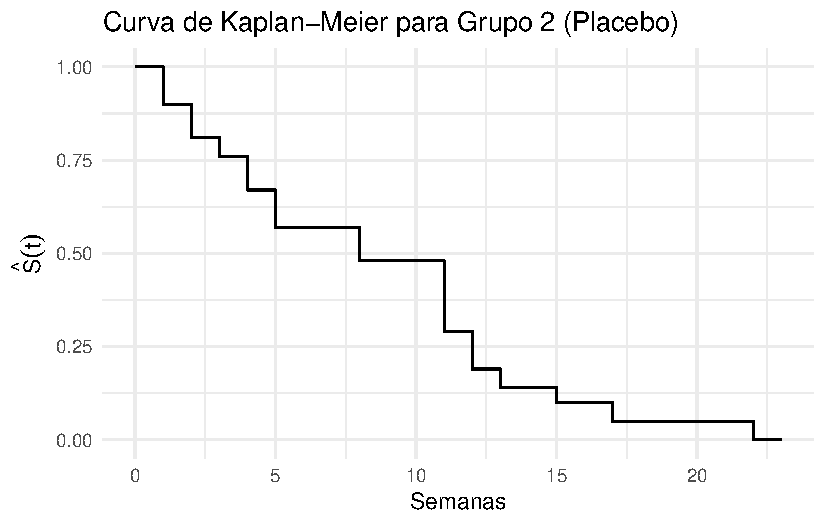
\includegraphics[keepaspectratio]{Unidad3_files/figure-pdf/unnamed-chunk-11-1.pdf}}

\begin{tcolorbox}[enhanced jigsaw, rightrule=.15mm, toprule=.15mm, colback=white, bottomrule=.15mm, bottomtitle=1mm, left=2mm, leftrule=.75mm, arc=.35mm, breakable, title=\textcolor{quarto-callout-note-color}{\faInfo}\hspace{0.5em}{Interpretación}, opacitybacktitle=0.6, colframe=quarto-callout-note-color-frame, opacityback=0, toptitle=1mm, coltitle=black, titlerule=0mm, colbacktitle=quarto-callout-note-color!10!white]

\begin{itemize}
\tightlist
\item
  \(\hat{S}(t_{(f)}) = \dfrac{\text{Número de sujetos sobrevivientes después de } t_{(f)}}{21}\)
\item
  No hay censura en el Grupo 2.
\item
  Se utilizó el método de Kaplan-Meier para estimar la función de
  supervivencia.
\end{itemize}

\end{tcolorbox}

\begin{center}\rule{0.5\linewidth}{0.5pt}\end{center}

\begin{tcolorbox}[enhanced jigsaw, rightrule=.15mm, toprule=.15mm, colback=white, bottomrule=.15mm, bottomtitle=1mm, left=2mm, leftrule=.75mm, arc=.35mm, breakable, title=\textcolor{quarto-callout-note-color}{\faInfo}\hspace{0.5em}{Ejemplo: Cálculo de la función de supervivencia empírica}, opacitybacktitle=0.6, colframe=quarto-callout-note-color-frame, opacityback=0, toptitle=1mm, coltitle=black, titlerule=0mm, colbacktitle=quarto-callout-note-color!10!white]

\begin{longtable}[]{@{}rrrrl@{}}
\caption{Grupo 2 (placebo): Estimación de la función de supervivencia
empírica (Kaplan-Meier)}\tabularnewline
\toprule\noalign{}
\(t_{(f)}\) & \(n_f\) & \(m_f\) & \(q_f\) & \(\hat{S}(t_{(f)})\) \\
\midrule\noalign{}
\endfirsthead
\toprule\noalign{}
\(t_{(f)}\) & \(n_f\) & \(m_f\) & \(q_f\) & \(\hat{S}(t_{(f)})\) \\
\midrule\noalign{}
\endhead
\bottomrule\noalign{}
\endlastfoot
0 & 21 & 0 & 0 & 1.00 \\
1 & 21 & 2 & 0 & 0.90 \\
2 & 19 & 2 & 0 & 0.81 \\
3 & 17 & 1 & 0 & 0.76 \\
4 & 16 & 2 & 0 & 0.67 \\
5 & 14 & 2 & 0 & 0.57 \\
8 & 12 & 4 & 0 & 0.48 \\
11 & 8 & 2 & 0 & 0.29 \\
12 & 6 & 2 & 0 & 0.19 \\
13 & 4 & 1 & 0 & 0.14 \\
15 & 3 & 1 & 0 & 0.10 \\
17 & 2 & 1 & 0 & 0.05 \\
22 & 1 & 1 & 0 & 0.00 \\
23 & 1 & 1 & 0 & 0.00 \\
\end{longtable}

Sea \(\hat{S}(4)\) la probabilidad estimada de supervivencia más allá de
la semana 4:

\[
\hat{S}(4) = 1 \times \frac{19}{21} \times \frac{17}{19} \times \frac{16}{17} \times \frac{14}{16} = \frac{14}{21} = 0.67
\]

Esto equivale a:

\begin{itemize}
\tightlist
\item
  \(\Pr(T > t_{(0)}) = \frac{21}{21}=1\)
\item
  \(\Pr(T > t_{(1)} \mid T \ge t_{(1)}) = \frac{19}{21}\)
\item
  \(\Pr(T > t_{(2)} \mid T \ge t_{(2)}) = \frac{19}{19}\)
\item
  \(\Pr(T > t_{(3)} \mid T \ge t_{(3)}) = \frac{16}{17}\)
\item
  \(\Pr(T > t_{(4)} \mid T \ge t_{(4)}) = \frac{14}{16}\)
\end{itemize}

Donde \(16\) es el número de individuos en riesgo en la semana 4.

Para \(t = 8\):

\[
\hat{S}(8) = 1 \times \frac{19}{21} \times \frac{17}{19} \times \frac{16}{17} \times \frac{14}{16} \times \frac{12}{14} \times \frac{8}{12} = \frac{8}{21}
\]

\end{tcolorbox}

\textbf{Fórmula KM:}\\
\[
\hat{S}(t) = \prod_{t_{(j)} \le t} \left( 1 - \frac{m_j}{n_j} \right)
\] donde \(m_j\) es el número de eventos (fallos) en \(t_{(j)}\) y
\(n_j\) el número en riesgo.

\begin{center}\rule{0.5\linewidth}{0.5pt}\end{center}

\begin{longtable}[]{@{}lrrrl@{}}
\caption{Grupo 1 (tratamiento): Estimación paso a paso de la función de
supervivencia KM}\tabularnewline
\toprule\noalign{}
\(t_{(f)}\) & \(n_f\) & \(m_f\) & \(q_f\) & \(\hat{S}(t_{(f)})\) \\
\midrule\noalign{}
\endfirsthead
\toprule\noalign{}
\(t_{(f)}\) & \(n_f\) & \(m_f\) & \(q_f\) & \(\hat{S}(t_{(f)})\) \\
\midrule\noalign{}
\endhead
\bottomrule\noalign{}
\endlastfoot
0 & 21 & 0 & 0 & 1 \\
6 & 21 & 3 & 1 & 18/21 = 0.8571 \\
7 & 17 & 1 & 1 & 0.8571 × 16/17 = 0.8067 \\
10 & 15 & 1 & 2 & 0.8067 × 14/15 = 0.7529 \\
13 & 12 & 1 & 1 & 0.7529 × 11/12 = 0.6902 \\
16 & 11 & 1 & 2 & 0.6902 × 10/11 = 0.6275 \\
22 & 7 & 1 & 1 & 0.6275 × 6/7 = 0.5378 \\
23 & 6 & 1 & 1 & 0.5378 × 5/6 = 0.4482 \\
\end{longtable}

\begin{tcolorbox}[enhanced jigsaw, rightrule=.15mm, toprule=.15mm, colback=white, bottomrule=.15mm, bottomtitle=1mm, left=2mm, leftrule=.75mm, arc=.35mm, breakable, title=\textcolor{quarto-callout-note-color}{\faInfo}\hspace{0.5em}{Cálculo de otras estimaciones de supervivencia}, opacitybacktitle=0.6, colframe=quarto-callout-note-color-frame, opacityback=0, toptitle=1mm, coltitle=black, titlerule=0mm, colbacktitle=quarto-callout-note-color!10!white]

Las demás estimaciones de supervivencia se calculan multiplicando la
estimación en el tiempo de fallo inmediatamente anterior por una
fracción.

Por ejemplo:

\begin{itemize}
\tightlist
\item
  La fracción es \(\frac{18}{21}\) para sobrevivir más allá de la semana
  6, porque 21 sujetos permanecen hasta la semana 6 y 3 de ellos no
  sobreviven más allá de esa semana.
\item
  La fracción es \(\frac{16}{17}\) para sobrevivir más allá de la semana
  7, ya que 17 personas permanecen hasta la semana 7 y 1 de ellas no
  sobrevive más allá de esa semana.
\end{itemize}

Las demás fracciones se calculan de manera similar.

\end{tcolorbox}

\begin{center}\rule{0.5\linewidth}{0.5pt}\end{center}

\pandocbounded{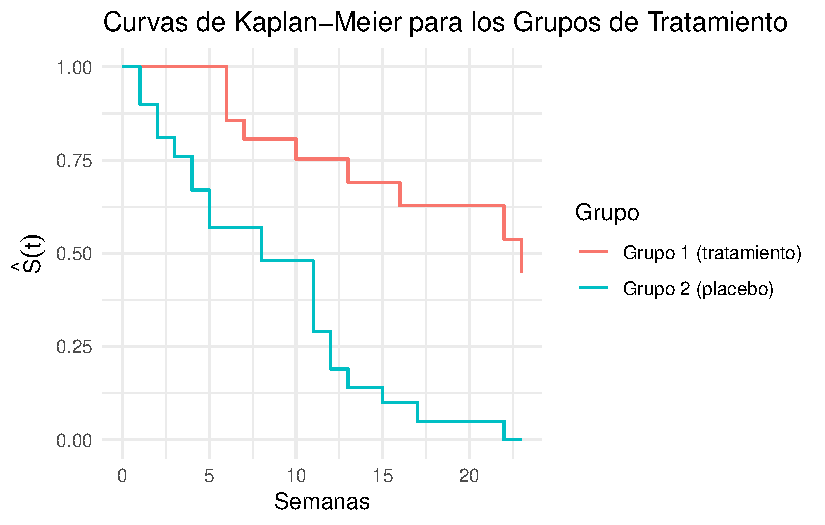
\includegraphics[keepaspectratio]{Unidad3_files/figure-pdf/unnamed-chunk-14-1.pdf}}

\subsection{III. Características Generales de las Curvas de
Kaplan-Meier}\label{iii.-caracteruxedsticas-generales-de-las-curvas-de-kaplan-meier}

\subsubsection{Fórmula general de KM}\label{fuxf3rmula-general-de-km}

\[
\hat{S}(t_{(f)}) = \hat{S}(t_{(f-1)}) \times \Pr(T > t_{(f)} \mid T \ge t_{(f)})
\]

\subsubsection{Fórmula producto-límite
(KM)}\label{fuxf3rmula-producto-luxedmite-km}

\[
\hat{S}(t_{(f)}) = \prod_{i=1}^{f} \Pr(T > t_{(i)} \mid T \ge t_{(i)})
\]

\begin{center}\rule{0.5\linewidth}{0.5pt}\end{center}

\subsubsection{Ejemplo}\label{ejemplo}

\begin{longtable}[]{@{}lrrrl@{}}
\caption{Grupo 1 (tratamiento): Estimación paso a paso de la función de
supervivencia KM}\tabularnewline
\toprule\noalign{}
\(t_{(f)}\) & \(n_f\) & \(m_f\) & \(q_f\) & \(\hat{S}(t_{(f)})\) \\
\midrule\noalign{}
\endfirsthead
\toprule\noalign{}
\(t_{(f)}\) & \(n_f\) & \(m_f\) & \(q_f\) & \(\hat{S}(t_{(f)})\) \\
\midrule\noalign{}
\endhead
\bottomrule\noalign{}
\endlastfoot
0 & 21 & 0 & 0 & 1 \\
6 & 21 & 3 & 1 & 18/21 = 0.8571 \\
7 & 17 & 1 & 1 & 0.8571 × 16/17 = 0.8067 \\
10 & 15 & 1 & 2 & 0.8067 × 14/15 = 0.7529 \\
13 & 12 & 1 & 1 & 0.7529 × 11/12 = 0.6902 \\
16 & 11 & 1 & 2 & 0.6902 × 10/11 = 0.6275 \\
22 & 7 & 1 & 1 & 0.6275 × 6/7 = 0.5378 \\
23 & 6 & 1 & 1 & 0.5378 × 5/6 = 0.4482 \\
\end{longtable}

\paragraph{\texorpdfstring{Para
\(t = 10\):}{Para t = 10:}}\label{para-t-10}

\[
\hat{S}(10) = 0.8067 \times \frac{14}{15} = 0.7529
\]

También se puede expresar como:

\[
\hat{S}(10) = \frac{18}{21} \times \frac{16}{17} \times \frac{14}{15}
\]

\paragraph{\texorpdfstring{Para
\(t = 16\):}{Para t = 16:}}\label{para-t-16}

\[
\hat{S}(16) = 0.6902 \times \frac{10}{11} = 0.6274
\]

O bien:

\[
\hat{S}(16) = \frac{18}{21} \times \frac{16}{17} \times \frac{14}{15} \times \frac{11}{12} \times \frac{10}{11}
\]

\subsection{Justificación Matemática de la Fórmula
KM}\label{justificaciuxf3n-matemuxe1tica-de-la-fuxf3rmula-km}

Sea:

\begin{itemize}
\tightlist
\item
  \(A = \{T \ge t_{(f)}\}\)
\item
  \(B = \{T > t_{(f)}\}\)
\end{itemize}

Entonces:

\[
\Pr(A \cap B) = \Pr(B) = \hat{S}(t_{(f)})
\]

Dado que no hay fallos en \(t_{(f-1)} < T < t_{(f)}\):

\[
\Pr(A) = \Pr(T \ge t_{(f-1)}) = \hat{S}(t_{(f-1)})
\]

Y por la regla de la probabilidad condicional:

\[
\Pr(B \mid A) = \Pr(T > t_{(f)} \mid T \ge t_{(f)})
\]

Por lo tanto, usando \(\Pr(A \cap B) = \Pr(A) \cdot \Pr(B \mid A)\):

\[
\hat{S}(t_{(f)}) = \hat{S}(t_{(f-1)}) \cdot \Pr(T > t_{(f)} \mid T \ge t_{(f)})
\]

\begin{center}\rule{0.5\linewidth}{0.5pt}\end{center}

\subsection{Ejemplo en R: Kaplan-Meier}\label{ejemplo-en-r-kaplan-meier}

\begin{longtable}[]{@{}lrr@{}}
\caption{Tabla de tiempos y estatus de censura}\tabularnewline
\toprule\noalign{}
ID & tiempo & evento \\
\midrule\noalign{}
\endfirsthead
\toprule\noalign{}
ID & tiempo & evento \\
\midrule\noalign{}
\endhead
\bottomrule\noalign{}
\endlastfoot
Ind 1 & 2.0 & 1 \\
Ind 2 & 3.0 & 1 \\
Ind 3 & 4.0 & 1 \\
Ind 4 & 4.5 & 0 \\
Ind 5 & 6.0 & 1 \\
Ind 6 & 7.0 & 1 \\
Ind 7 & 9.0 & 0 \\
Ind 8 & 10.0 & 1 \\
\end{longtable}

\pandocbounded{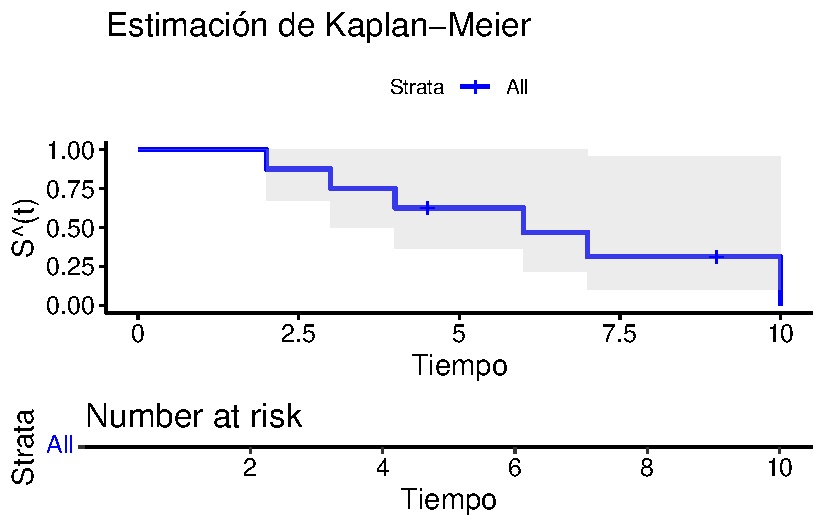
\includegraphics[keepaspectratio]{Unidad3_files/figure-pdf/unnamed-chunk-17-1.pdf}}

\begin{verbatim}
Call: survfit(formula = surv_obj ~ 1, data = datos)

 time n.risk n.event survival std.err lower 95% CI upper 95% CI
    2      8       1    0.875   0.117        0.673        1.000
    3      7       1    0.750   0.153        0.503        1.000
    4      6       1    0.625   0.171        0.365        1.000
    6      4       1    0.469   0.187        0.215        1.000
    7      3       1    0.312   0.178        0.102        0.955
   10      1       1    0.000     NaN           NA           NA
\end{verbatim}

\section{Aplicación}\label{aplicaciuxf3n}

\subsection{Uso en R}\label{uso-en-r}

\begin{itemize}
\tightlist
\item
  Librería \texttt{survival}:
\end{itemize}

\begin{Shaded}
\begin{Highlighting}[]
\FunctionTok{library}\NormalTok{(survival)}
\FunctionTok{Surv}\NormalTok{(tiempo, status)}
\end{Highlighting}
\end{Shaded}

\begin{itemize}
\tightlist
\item
  Este objeto puede usarse en:

  \begin{itemize}
  \tightlist
  \item
    \href{https://www.rdocumentation.org/packages/survival/versions/3.5-7/topics/Surv}{Surv()}
    codifica la información de tiempo y censura.
  \item
    \href{https://www.rdocumentation.org/packages/survival/versions/3.8-3/topics/survfit.formula}{survfit()}
    ajusta curvas de supervivencia (Kaplan-Meier).
  \item
    \href{https://www.rdocumentation.org/packages/survival/versions/3.5-7/topics/coxph}{coxph()}
    para modelos de Cox
  \end{itemize}
\end{itemize}

\begin{center}\rule{0.5\linewidth}{0.5pt}\end{center}

\subsubsection{\texorpdfstring{La función \texttt{Surv()} de
\texttt{survival}}{La función Surv() de survival}}\label{la-funciuxf3n-surv-de-survival}

\begin{Shaded}
\begin{Highlighting}[]
\FunctionTok{library}\NormalTok{(survival)}

\CommentTok{\# Censura derecha}
\NormalTok{tiempos }\OtherTok{\textless{}{-}} \FunctionTok{c}\NormalTok{(}\DecValTok{5}\NormalTok{, }\DecValTok{8}\NormalTok{, }\DecValTok{12}\NormalTok{, }\DecValTok{3}\NormalTok{, }\DecValTok{10}\NormalTok{)}
\NormalTok{evento }\OtherTok{\textless{}{-}} \FunctionTok{c}\NormalTok{(}\DecValTok{1}\NormalTok{, }\DecValTok{0}\NormalTok{, }\DecValTok{1}\NormalTok{, }\DecValTok{1}\NormalTok{, }\DecValTok{0}\NormalTok{)  }\CommentTok{\# 1 = evento, 0 = censurado}

\NormalTok{datos }\OtherTok{\textless{}{-}} \FunctionTok{Surv}\NormalTok{(tiempos, evento)}
\NormalTok{datos}
\end{Highlighting}
\end{Shaded}

\begin{verbatim}
[1]  5   8+ 12   3  10+
\end{verbatim}

\begin{itemize}
\tightlist
\item
  Crea un objeto de clase \texttt{Surv}.
\item
  Es la base para ajustar modelos de supervivencia.
\end{itemize}

\subsubsection{\texorpdfstring{Visualizando \texttt{Surv()} con tipos de
censura}{Visualizando Surv() con tipos de censura}}\label{visualizando-surv-con-tipos-de-censura}

\begin{Shaded}
\begin{Highlighting}[]
\CommentTok{\# Censura izquierda}
\NormalTok{tiempos }\OtherTok{\textless{}{-}} \FunctionTok{c}\NormalTok{(}\DecValTok{5}\NormalTok{, }\DecValTok{8}\NormalTok{, }\DecValTok{12}\NormalTok{, }\DecValTok{3}\NormalTok{, }\DecValTok{10}\NormalTok{)}
\NormalTok{evento }\OtherTok{\textless{}{-}} \FunctionTok{c}\NormalTok{(}\DecValTok{1}\NormalTok{, }\DecValTok{0}\NormalTok{, }\DecValTok{1}\NormalTok{, }\DecValTok{1}\NormalTok{, }\DecValTok{0}\NormalTok{)}
\FunctionTok{Surv}\NormalTok{(tiempos, evento, }\AttributeTok{type =} \StringTok{"left"}\NormalTok{)}
\end{Highlighting}
\end{Shaded}

\begin{verbatim}
[1]  5   8- 12   3  10-
\end{verbatim}

\begin{Shaded}
\begin{Highlighting}[]
\CommentTok{\# Censura por intervalo}
\NormalTok{inferior }\OtherTok{\textless{}{-}} \FunctionTok{c}\NormalTok{(}\DecValTok{2}\NormalTok{, }\DecValTok{6}\NormalTok{, }\DecValTok{7}\NormalTok{, }\DecValTok{5}\NormalTok{, }\DecValTok{1}\NormalTok{)}
\NormalTok{superior }\OtherTok{\textless{}{-}} \FunctionTok{c}\NormalTok{(}\DecValTok{4}\NormalTok{, }\DecValTok{6}\NormalTok{, }\DecValTok{9}\NormalTok{, }\DecValTok{6}\NormalTok{, }\DecValTok{3}\NormalTok{)}
\NormalTok{evento }\OtherTok{\textless{}{-}} \FunctionTok{c}\NormalTok{(}\DecValTok{3}\NormalTok{, }\DecValTok{0}\NormalTok{, }\DecValTok{3}\NormalTok{, }\DecValTok{0}\NormalTok{, }\DecValTok{3}\NormalTok{)  }\CommentTok{\# 3 = intervalo}
\FunctionTok{Surv}\NormalTok{(inferior, superior, }\AttributeTok{type =} \StringTok{"interval2"}\NormalTok{)}
\end{Highlighting}
\end{Shaded}

\begin{verbatim}
[1] [2, 4] 6      [7, 9] [5, 6] [1, 3]
\end{verbatim}

\begin{center}\rule{0.5\linewidth}{0.5pt}\end{center}

\subsubsection{\texorpdfstring{Ajuste con
\texttt{survfit()}}{Ajuste con survfit()}}\label{ajuste-con-survfit}

\begin{Shaded}
\begin{Highlighting}[]
\FunctionTok{library}\NormalTok{(survival)}

\CommentTok{\# Datos con censura derecha}
\NormalTok{tiempos }\OtherTok{\textless{}{-}} \FunctionTok{c}\NormalTok{(}\DecValTok{5}\NormalTok{, }\DecValTok{8}\NormalTok{, }\DecValTok{12}\NormalTok{, }\DecValTok{3}\NormalTok{, }\DecValTok{10}\NormalTok{)}
\NormalTok{evento }\OtherTok{\textless{}{-}} \FunctionTok{c}\NormalTok{(}\DecValTok{1}\NormalTok{, }\DecValTok{0}\NormalTok{, }\DecValTok{1}\NormalTok{, }\DecValTok{1}\NormalTok{, }\DecValTok{0}\NormalTok{)}
\NormalTok{datos }\OtherTok{\textless{}{-}} \FunctionTok{Surv}\NormalTok{(tiempos, evento)}
\FunctionTok{print}\NormalTok{(datos)}
\end{Highlighting}
\end{Shaded}

\begin{verbatim}
[1]  5   8+ 12   3  10+
\end{verbatim}

\begin{Shaded}
\begin{Highlighting}[]
\NormalTok{modelo }\OtherTok{\textless{}{-}} \FunctionTok{survfit}\NormalTok{(datos }\SpecialCharTok{\textasciitilde{}} \DecValTok{1}\NormalTok{)  }\CommentTok{\# sin covariables}
\FunctionTok{summary}\NormalTok{(modelo)}
\end{Highlighting}
\end{Shaded}

\begin{verbatim}
Call: survfit(formula = datos ~ 1)

 time n.risk n.event survival std.err lower 95% CI upper 95% CI
    3      5       1      0.8   0.179        0.516            1
    5      4       1      0.6   0.219        0.293            1
   12      1       1      0.0     NaN           NA           NA
\end{verbatim}

\begin{itemize}
\tightlist
\item
  \texttt{survfit()} ajusta una curva de Kaplan-Meier.
\end{itemize}

\begin{center}\rule{0.5\linewidth}{0.5pt}\end{center}

\subsubsection{Graficando la curva de
supervivencia}\label{graficando-la-curva-de-supervivencia}

\begin{Shaded}
\begin{Highlighting}[]
\FunctionTok{plot}\NormalTok{(modelo, }\AttributeTok{xlab =} \StringTok{"Tiempo"}\NormalTok{, }\AttributeTok{ylab =} \StringTok{"Supervivencia estimada"}\NormalTok{,}
     \AttributeTok{main =} \StringTok{"Curva de Kaplan{-}Meier"}\NormalTok{)}
\end{Highlighting}
\end{Shaded}

\pandocbounded{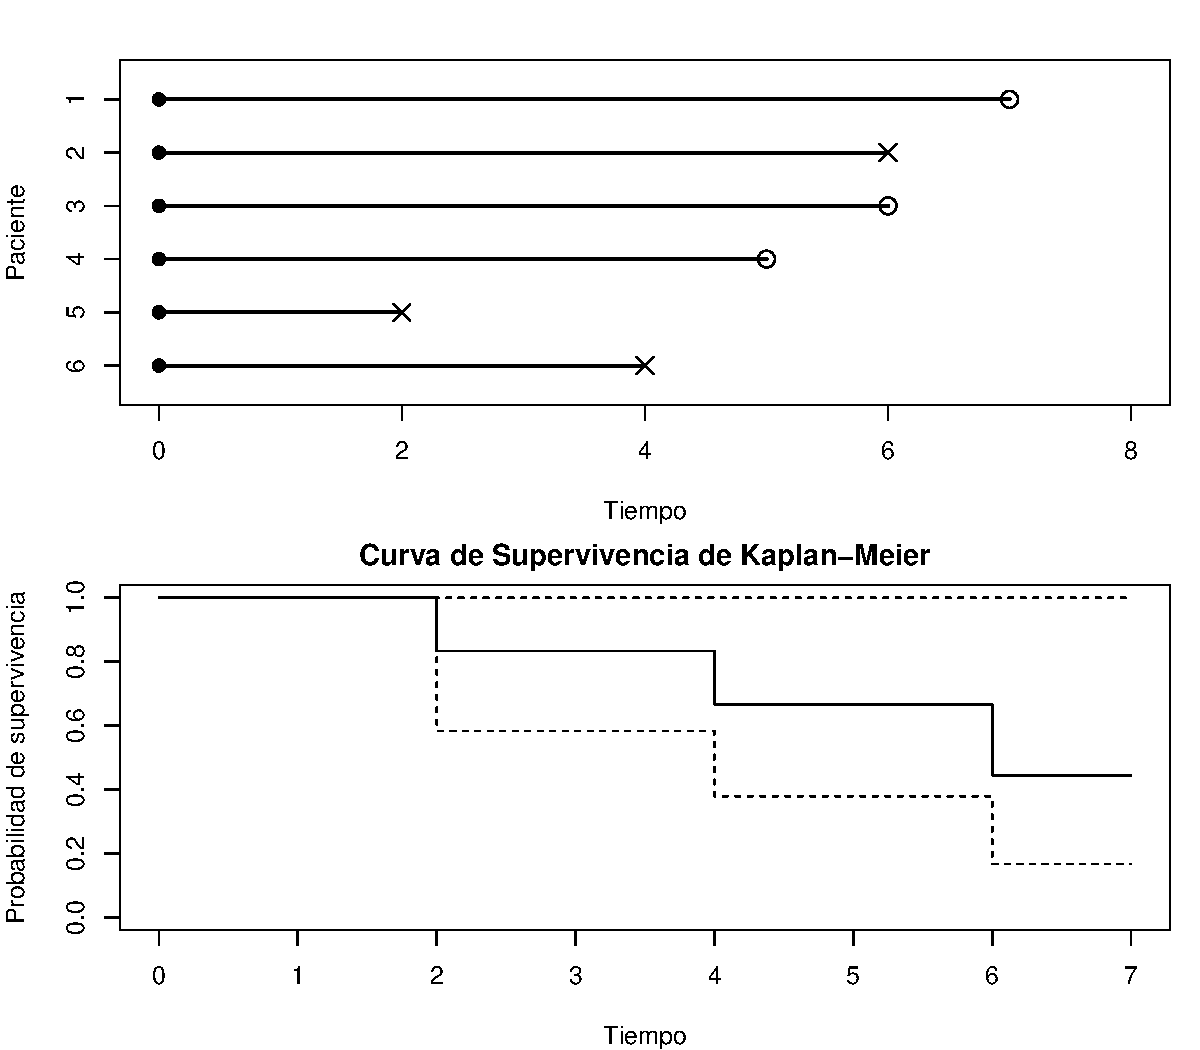
\includegraphics[keepaspectratio]{Unidad3_files/figure-pdf/unnamed-chunk-23-1.pdf}}

\begin{quote}
Puedes usar
\href{https://www.rdocumentation.org/packages/survminer/versions/0.4.9/topics/ggsurvplot}{ggsurvplot()}
del paquete \texttt{survminer} para una mejor presentación visual.
\end{quote}

\begin{center}\rule{0.5\linewidth}{0.5pt}\end{center}

\begin{Shaded}
\begin{Highlighting}[]
\NormalTok{survminer}\SpecialCharTok{::}\FunctionTok{ggsurvplot}\NormalTok{(modelo,}\AttributeTok{data=}\NormalTok{datos, }\AttributeTok{xlab =} \StringTok{"Tiempo"}\NormalTok{, }\AttributeTok{ylab =} \StringTok{"Supervivencia estimada"}\NormalTok{,}
     \AttributeTok{title =} \StringTok{"Curva de Kaplan{-}Meier"}\NormalTok{)}
\end{Highlighting}
\end{Shaded}

\pandocbounded{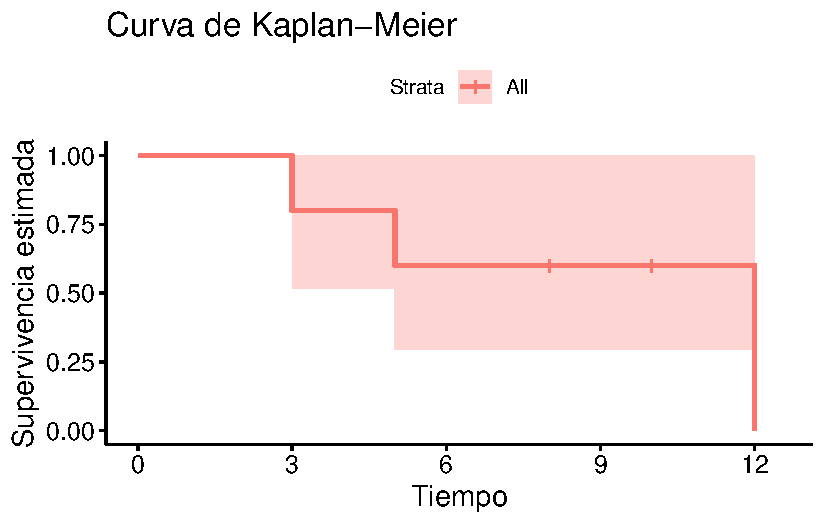
\includegraphics[keepaspectratio]{Unidad3_files/figure-pdf/unnamed-chunk-24-1.pdf}}

\section{Intervalo de Confianza en
Kaplan-Meier}\label{intervalo-de-confianza-en-kaplan-meier}

\subsection{Intervalo de Confianza en
Kaplan-Meier}\label{intervalo-de-confianza-en-kaplan-meier-1}

\begin{itemize}
\tightlist
\item
  La estimación de la supervivencia mediante Kaplan-Meier es una curva
  escalonada.
\item
  Cada punto de la curva tiene asociado un \textbf{intervalo de
  confianza (IC)}.
\item
  El IC refleja la \textbf{incertidumbre} de la estimación en cada
  tiempo debido a datos censurados y al tamaño muestral.
\end{itemize}

\begin{center}\rule{0.5\linewidth}{0.5pt}\end{center}

\subsection{Fórmula general del IC}\label{fuxf3rmula-general-del-ic}

Para una estimación de la probabilidad de supervivencia
\(\hat{S}_{KM}(t)\) en un tiempo `t' dado, el IC del 95\% se calcula
como:

\[
\hat{S}_{KM}(t) \pm 1.96 \cdot \sqrt{\text{Var}(\hat{S}_{KM}(t))}
\]

\begin{itemize}
\tightlist
\item
  \(\hat{S}_{KM}(t)\): estimador de Kaplan-Meier
\item
  \(\text{Var}(\hat{S}_{KM}(t))\): varianza estimada con la fórmula de
  Greenwood, Ver sección 4.4 de Klein \& Moeschberger (2003) para
  detalles sobre la fórmula de Greenwood.
\item
  \(1.96\): cuantil de la normal estándar para un 95\% de confianza
\end{itemize}

\begin{center}\rule{0.5\linewidth}{0.5pt}\end{center}

\subsection{Fórmula de Greenwood para la
Varianza}\label{fuxf3rmula-de-greenwood-para-la-varianza}

\[
\text{Var}(\hat{S}(t)) = [\hat{S}(t)]^2 \cdot \sum_{j: t_j \leq t} \frac{m_j}{n_j(n_j - m_j)}
\]

Donde:

\begin{itemize}
\tightlist
\item
  \(m_j\): número de fallas en el tiempo \(t_j\)
\item
  \(n_j\): número de sujetos en riesgo justo antes de \(t_j\)
\end{itemize}

\begin{center}\rule{0.5\linewidth}{0.5pt}\end{center}

\subsection{Ejemplo de cálculo}\label{ejemplo-de-cuxe1lculo}

\begin{longtable}[]{@{}
  >{\raggedleft\arraybackslash}p{(\linewidth - 14\tabcolsep) * \real{0.0370}}
  >{\raggedright\arraybackslash}p{(\linewidth - 14\tabcolsep) * \real{0.0741}}
  >{\raggedleft\arraybackslash}p{(\linewidth - 14\tabcolsep) * \real{0.0741}}
  >{\raggedleft\arraybackslash}p{(\linewidth - 14\tabcolsep) * \real{0.0741}}
  >{\raggedright\arraybackslash}p{(\linewidth - 14\tabcolsep) * \real{0.1605}}
  >{\raggedright\arraybackslash}p{(\linewidth - 14\tabcolsep) * \real{0.1852}}
  >{\raggedright\arraybackslash}p{(\linewidth - 14\tabcolsep) * \real{0.1975}}
  >{\raggedright\arraybackslash}p{(\linewidth - 14\tabcolsep) * \real{0.1975}}@{}}
\caption{Tabla completa con eventos y censuras para los 21
casos}\tabularnewline
\toprule\noalign{}
\begin{minipage}[b]{\linewidth}\raggedleft
t
\end{minipage} & \begin{minipage}[b]{\linewidth}\raggedright
\(n_f\)
\end{minipage} & \begin{minipage}[b]{\linewidth}\raggedleft
\(m_f\)
\end{minipage} & \begin{minipage}[b]{\linewidth}\raggedleft
\(q_f\)
\end{minipage} & \begin{minipage}[b]{\linewidth}\raggedright
\(\hat{S}(t)\)
\end{minipage} & \begin{minipage}[b]{\linewidth}\raggedright
Error estándar
\end{minipage} & \begin{minipage}[b]{\linewidth}\raggedright
Límite inferior
\end{minipage} & \begin{minipage}[b]{\linewidth}\raggedright
Límite superior
\end{minipage} \\
\midrule\noalign{}
\endfirsthead
\toprule\noalign{}
\begin{minipage}[b]{\linewidth}\raggedleft
t
\end{minipage} & \begin{minipage}[b]{\linewidth}\raggedright
\(n_f\)
\end{minipage} & \begin{minipage}[b]{\linewidth}\raggedleft
\(m_f\)
\end{minipage} & \begin{minipage}[b]{\linewidth}\raggedleft
\(q_f\)
\end{minipage} & \begin{minipage}[b]{\linewidth}\raggedright
\(\hat{S}(t)\)
\end{minipage} & \begin{minipage}[b]{\linewidth}\raggedright
Error estándar
\end{minipage} & \begin{minipage}[b]{\linewidth}\raggedright
Límite inferior
\end{minipage} & \begin{minipage}[b]{\linewidth}\raggedright
Límite superior
\end{minipage} \\
\midrule\noalign{}
\endhead
\bottomrule\noalign{}
\endlastfoot
6 & 21 & 3 & 1 & 0.857 & 0.0764 & 0.72 & 1 \\
7 & 17 & 1 & 0 & 0.807 & 0.0869 & 0.653 & 0.996 \\
9 & & 0 & 1 & & & & \\
10 & 15 & 1 & 1 & 0.753 & 0.0963 & 0.586 & 0.968 \\
11 & & 0 & 1 & & & & \\
13 & 12 & 1 & 0 & 0.69 & 0.1068 & 0.51 & 0.935 \\
16 & 11 & 1 & 0 & 0.627 & 0.1141 & 0.439 & 0.896 \\
17 & & 0 & 1 & & & & \\
19 & & 0 & 1 & & & & \\
20 & & 0 & 1 & & & & \\
22 & 7 & 1 & 0 & 0.538 & 0.1282 & 0.337 & 0.858 \\
23 & 6 & 1 & 0 & 0.448 & 0.1346 & 0.249 & 0.807 \\
25 & & 0 & 1 & & & & \\
32 & & 0 & 2 & & & & \\
34 & & 0 & 1 & & & & \\
35 & & 0 & 1 & & & & \\
\end{longtable}

\begin{itemize}
\tightlist
\item
  A las 10 semanas, \[\hat{S}(10) = 0.753\]
\item
  Eventos y riesgos previos:

  \begin{itemize}
  \tightlist
  \item
    Semana 6: \(m_f = 3, n_f = 21\) → \(\frac{3}{21 \cdot 18} = 0.0079\)
  \item
    Semana 7: \(m_f = 1, n_f = 18\) → \(\frac{1}{18 \cdot 17} = 0.0033\)
  \item
    Semana 10: \(m_f = 1, n_f = 17\) →
    \(\frac{1}{17 \cdot 16} = 0.0037\)
  \end{itemize}
\end{itemize}

\[
\sum = 0.0079+0.0033+0.0037=0.0149
\]

\[
\text{Var}(\hat{S}(10)) = (0.753)^2 \cdot 0.0149=0.0084
\]

IC del 95\%: \[
0.753 \pm 1.96 \cdot \sqrt{0.0084} = (0.570, 0.936)
\]

\begin{center}\rule{0.5\linewidth}{0.5pt}\end{center}

\subsection{Visualización en R}\label{visualizaciuxf3n-en-r}

\begin{Shaded}
\begin{Highlighting}[]
\FunctionTok{library}\NormalTok{(survival)}

\NormalTok{tratamiento }\OtherTok{\textless{}{-}} \FunctionTok{data.frame}\NormalTok{(}\AttributeTok{tiempo =} \FunctionTok{c}\NormalTok{(}\DecValTok{6}\NormalTok{, }\DecValTok{6}\NormalTok{, }\DecValTok{6}\NormalTok{, }\DecValTok{7}\NormalTok{, }\DecValTok{10}\NormalTok{, }\DecValTok{13}\NormalTok{, }\DecValTok{16}\NormalTok{, }\DecValTok{22}\NormalTok{, }\DecValTok{23}\NormalTok{, }
                               \DecValTok{6}\NormalTok{, }\DecValTok{9}\NormalTok{, }\DecValTok{10}\NormalTok{, }\DecValTok{11}\NormalTok{, }\DecValTok{17}\NormalTok{, }\DecValTok{19}\NormalTok{, }\DecValTok{20}\NormalTok{, }\DecValTok{25}\NormalTok{, }\DecValTok{32}\NormalTok{, }\DecValTok{32}\NormalTok{, }\DecValTok{34}\NormalTok{, }\DecValTok{35}\NormalTok{),}
                    \AttributeTok{status =} \FunctionTok{c}\NormalTok{(}\FunctionTok{rep}\NormalTok{(}\DecValTok{1}\NormalTok{,}\DecValTok{9}\NormalTok{),}\FunctionTok{rep}\NormalTok{(}\DecValTok{0}\NormalTok{,}\DecValTok{12}\NormalTok{)))}


\NormalTok{ajuste }\OtherTok{\textless{}{-}} \FunctionTok{survfit}\NormalTok{(}\FunctionTok{Surv}\NormalTok{(tiempo, status) }\SpecialCharTok{\textasciitilde{}} \DecValTok{1}\NormalTok{, }\AttributeTok{data =}\NormalTok{ tratamiento)}
\FunctionTok{summary}\NormalTok{(ajuste)}
\end{Highlighting}
\end{Shaded}

\begin{verbatim}
Call: survfit(formula = Surv(tiempo, status) ~ 1, data = tratamiento)

 time n.risk n.event survival std.err lower 95% CI upper 95% CI
    6     21       3    0.857  0.0764        0.720        1.000
    7     17       1    0.807  0.0869        0.653        0.996
   10     15       1    0.753  0.0963        0.586        0.968
   13     12       1    0.690  0.1068        0.510        0.935
   16     11       1    0.627  0.1141        0.439        0.896
   22      7       1    0.538  0.1282        0.337        0.858
   23      6       1    0.448  0.1346        0.249        0.807
\end{verbatim}

\begin{Shaded}
\begin{Highlighting}[]
\FunctionTok{ggsurvplot}\NormalTok{(}\AttributeTok{fit=}\NormalTok{ajuste,}\AttributeTok{data=}\NormalTok{tratamiento)}
\end{Highlighting}
\end{Shaded}

\pandocbounded{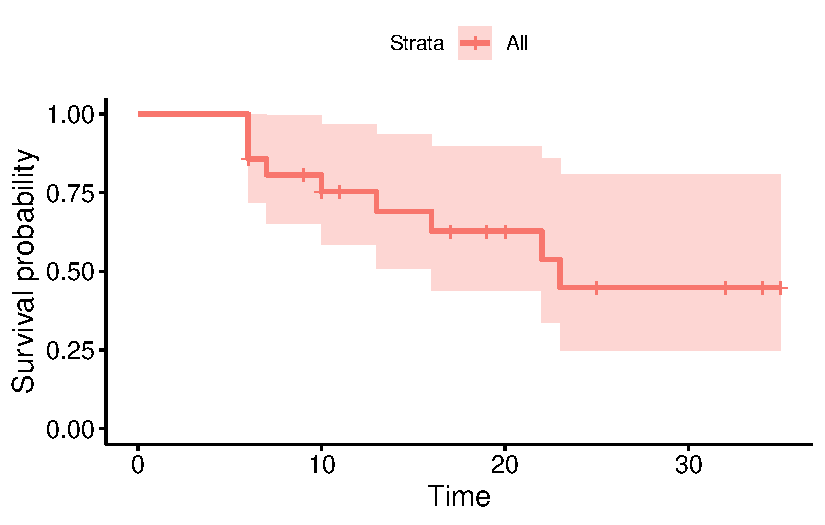
\includegraphics[keepaspectratio]{Unidad3_files/figure-pdf/unnamed-chunk-26-1.pdf}}

\begin{center}\rule{0.5\linewidth}{0.5pt}\end{center}

\subsection{Consideraciones finales de los intervalos de
confianza}\label{consideraciones-finales-de-los-intervalos-de-confianza}

\begin{itemize}
\tightlist
\item
  Los IC permiten visualizar la precisión de las curvas de
  supervivencia.
\item
  Son especialmente útiles para comparar entre grupos.
\end{itemize}

\section{Supervivencia Mediana}\label{supervivencia-mediana}

\subsection{¿Qué es la supervivencia
mediana?}\label{quuxe9-es-la-supervivencia-mediana}

\begin{itemize}
\tightlist
\item
  Es el tiempo en el cual la \textbf{probabilidad de supervivencia} se
  reduce al \textbf{50\%}.
\item
  También se define como el tiempo \texttt{t} tal que \[S(t) = 0.5\].
\item
  Es preferida sobre la \textbf{media} cuando hay datos
  \textbf{censurados}, ya que la media puede no estar bien definida si
  la cola derecha no está completamente observada.
\end{itemize}

\begin{center}\rule{0.5\linewidth}{0.5pt}\end{center}

\subsection{Ejemplo visual}\label{ejemplo-visual}

\pandocbounded{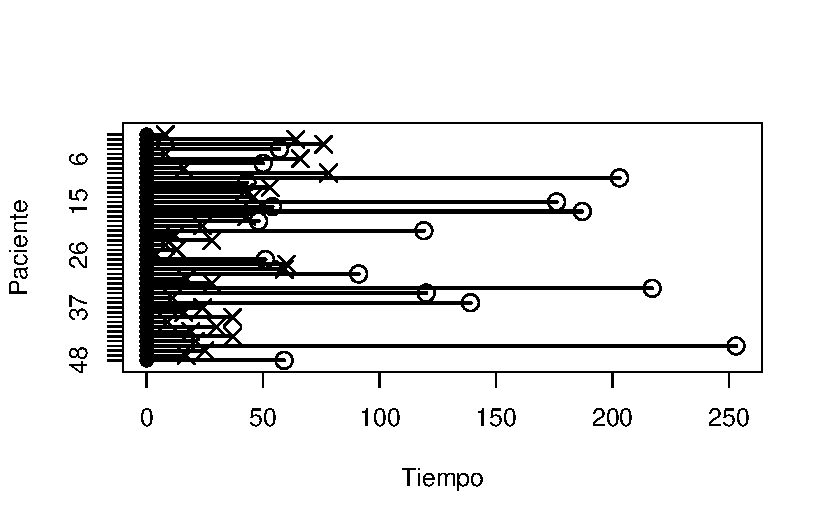
\includegraphics[keepaspectratio]{Unidad3_files/figure-pdf/unnamed-chunk-27-1.pdf}}

\begin{center}\rule{0.5\linewidth}{0.5pt}\end{center}

\subsection{¿Por qué es útil?}\label{por-quuxe9-es-uxfatil}

\begin{itemize}
\tightlist
\item
  Es \textbf{robusta} frente a valores extremos.
\item
  Resume la distribución del tiempo hasta el evento.
\item
  Tiene una \textbf{interpretación clara}: la mitad de los individuos
  han experimentado el evento para ese tiempo.
\end{itemize}

\begin{center}\rule{0.5\linewidth}{0.5pt}\end{center}

\subsection{Cálculo en R}\label{cuxe1lculo-en-r}

\begin{Shaded}
\begin{Highlighting}[]
\FunctionTok{summary}\NormalTok{(ajuste)}\SpecialCharTok{$}\NormalTok{table[}\StringTok{"median"}\NormalTok{]}
\end{Highlighting}
\end{Shaded}

\begin{verbatim}
  median 
11.00339 
\end{verbatim}

\begin{Shaded}
\begin{Highlighting}[]
\FunctionTok{print}\NormalTok{(ajuste)}
\end{Highlighting}
\end{Shaded}

\begin{verbatim}
Call: survfit(formula = surv_obj ~ 1)

      n events median 0.95LCL 0.95UCL
[1,] 50     36     11    7.91    15.6
\end{verbatim}

Este valor representa la \textbf{supervivencia mediana} estimada a
partir de los datos.

\begin{center}\rule{0.5\linewidth}{0.5pt}\end{center}

\subsection{\texorpdfstring{Conjunto de datos \texttt{gastricXelox} de
la biblioteca
\texttt{asaur}}{Conjunto de datos gastricXelox de la biblioteca asaur}}\label{conjunto-de-datos-gastricxelox-de-la-biblioteca-asaur}

\begin{Shaded}
\begin{Highlighting}[]
\FunctionTok{library}\NormalTok{(asaur)}
\FunctionTok{data}\NormalTok{(}\StringTok{"gastricXelox"}\NormalTok{)}
\end{Highlighting}
\end{Shaded}

\begin{longtable}[]{@{}rrr@{}}
\caption{Ejemplo}\tabularnewline
\toprule\noalign{}
paciente & tiempo & status \\
\midrule\noalign{}
\endfirsthead
\toprule\noalign{}
paciente & tiempo & status \\
\midrule\noalign{}
\endhead
\bottomrule\noalign{}
\endlastfoot
1 & 8 & 1 \\
2 & 64 & 1 \\
3 & 76 & 1 \\
4 & 57 & 0 \\
5 & 8 & 1 \\
6 & 66 & 1 \\
\end{longtable}

\begin{itemize}
\tightlist
\item
  Tiempo: semanas hasta progresión o muerte\\
\item
  \texttt{delta\ =\ 1} si hubo evento, \texttt{0} si censurado
\item
  Los datos se desordenaron para este ejemplo
\end{itemize}

\pandocbounded{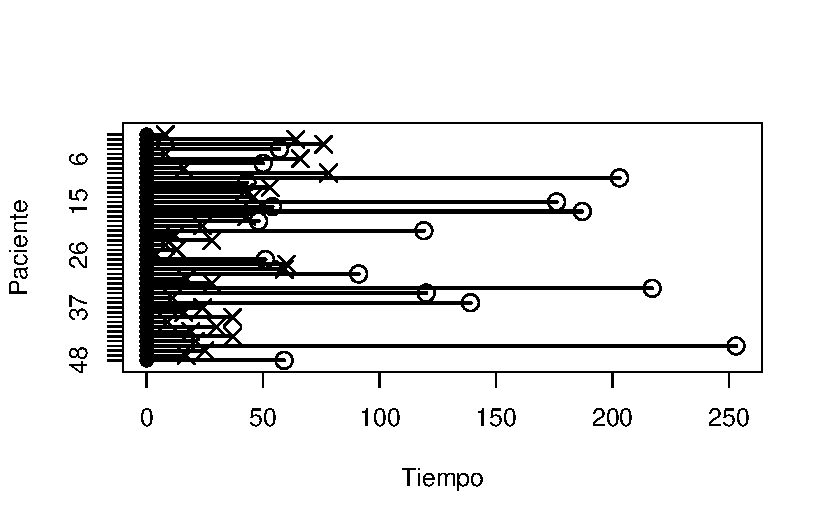
\includegraphics[keepaspectratio]{Unidad3_files/figure-pdf/unnamed-chunk-31-1.pdf}}

\pandocbounded{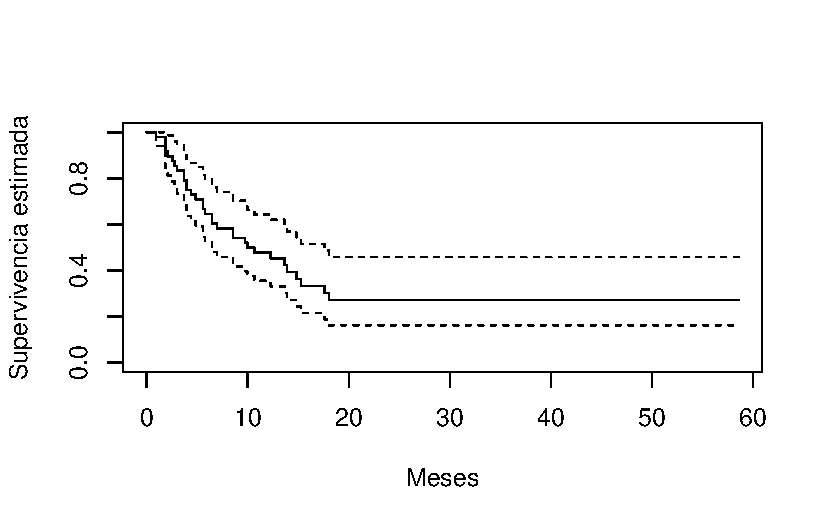
\includegraphics[keepaspectratio]{Unidad3_files/figure-pdf/unnamed-chunk-32-1.pdf}}

\begin{center}\rule{0.5\linewidth}{0.5pt}\end{center}

\subsection{Ejercicio}\label{ejercicio}

\begin{itemize}
\tightlist
\item
  Usar R para:

  \begin{itemize}
  \tightlist
  \item
    Estimar la curva de supervivencia de \texttt{gastricXelox}
  \item
    Obtener la mediana de supervivencia
  \item
    Graficar con intervalo de confianza
  \end{itemize}
\end{itemize}

\begin{verbatim}
Call: survfit(formula = Surv(timeMonths, delta) ~ 1, data = gastricXelox)

   time n.risk n.event survival std.err lower 95% CI upper 95% CI
  0.926     48       1    0.979  0.0206        0.940        1.000
  1.851     47       3    0.917  0.0399        0.842        0.998
  2.083     44       1    0.896  0.0441        0.813        0.987
  2.545     43       1    0.875  0.0477        0.786        0.974
  2.777     42       1    0.854  0.0509        0.760        0.960
  3.008     41       1    0.833  0.0538        0.734        0.946
  3.702     40       2    0.792  0.0586        0.685        0.915
  3.934     38       2    0.750  0.0625        0.637        0.883
  4.397     36       1    0.729  0.0641        0.614        0.866
  4.860     35       1    0.708  0.0656        0.591        0.849
  5.554     34       2    0.667  0.0680        0.546        0.814
  5.785     32       1    0.646  0.0690        0.524        0.796
  6.479     31       2    0.604  0.0706        0.481        0.760
  6.942     29       1    0.583  0.0712        0.459        0.741
  8.562     28       2    0.542  0.0719        0.418        0.703
  9.719     26       1    0.521  0.0721        0.397        0.683
  9.950     25       1    0.500  0.0722        0.377        0.663
 10.645     23       1    0.478  0.0722        0.356        0.643
 12.264     19       1    0.453  0.0727        0.331        0.620
 13.653     16       1    0.425  0.0735        0.303        0.596
 13.884     14       1    0.394  0.0742        0.273        0.570
 14.810     13       1    0.364  0.0744        0.244        0.544
 15.273     12       1    0.334  0.0742        0.216        0.516
 17.587     11       1    0.303  0.0734        0.189        0.487
 18.050     10       1    0.273  0.0720        0.163        0.458
\end{verbatim}

\pandocbounded{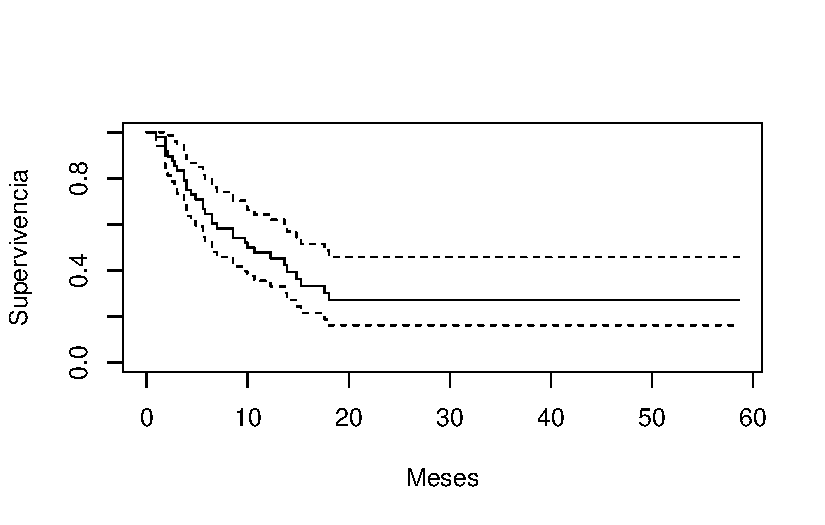
\includegraphics[keepaspectratio]{Unidad3_files/figure-pdf/unnamed-chunk-34-1.pdf}}

\section{Comparación entre grupos (Log-Rank
Test)}\label{comparaciuxf3n-entre-grupos-log-rank-test}

\subsection{Objetivo}\label{objetivo}

\begin{itemize}
\tightlist
\item
  Comparar curvas de supervivencia entre \textbf{dos o más grupos}.
\item
  Detectar diferencias globales en el riesgo de eventos a lo largo del
  tiempo.
\end{itemize}

\subsection{Hipótesis}\label{hipuxf3tesis}

\[
H_0: S_1(t) = S_2(t) \quad \forall t \\
H_A: S_1(t) \ne S_2(t) \quad \text{para al menos un valor de } t
\]

\begin{itemize}
\tightlist
\item
  Prueba \textbf{no paramétrica}
\item
  Se basa en la comparación entre \textbf{observados} y
  \textbf{esperados}
\end{itemize}

\begin{center}\rule{0.5\linewidth}{0.5pt}\end{center}

\subsection{Fundamento de la prueba}\label{fundamento-de-la-prueba}

En cada tiempo de fallo:

\begin{itemize}
\tightlist
\item
  Se registra el número de eventos observados (\(O_{1j}\), \(O_{2j}\))
\item
  Se calcula el número esperado bajo \(H_0\) (\(E_{1j}\), \(E_{2j}\))
\end{itemize}

Se acumulan a lo largo del tiempo:

\[
Z = \sum_j (O_{1j} - E_{1j})
\]

y la varianza:

\[
\text{Var}(Z) = \sum_j V_j
\]

\begin{center}\rule{0.5\linewidth}{0.5pt}\end{center}

\begin{tcolorbox}[enhanced jigsaw, rightrule=.15mm, toprule=.15mm, colback=white, bottomrule=.15mm, bottomtitle=1mm, left=2mm, leftrule=.75mm, arc=.35mm, breakable, title=\textcolor{quarto-callout-note-color}{\faInfo}\hspace{0.5em}{Cálculo del número esperado bajo \(H_0\)}, opacitybacktitle=0.6, colframe=quarto-callout-note-color-frame, opacityback=0, toptitle=1mm, coltitle=black, titlerule=0mm, colbacktitle=quarto-callout-note-color!10!white]

En la prueba de log-rank, bajo la hipótesis nula
\(H_0: S_1(t) = S_2(t)\), se asume que \textbf{las tasas de fallo son
iguales en ambos grupos}. Por tanto, el número esperado de fallos para
cada grupo en el tiempo de fallo \(t_{(f)}\) se calcula como:

\begin{itemize}
\item
  Número total de fallos en \(t_{(f)}\):\\
  \[
  m_f = m_{1f} + m_{2f}
  \]
\item
  Número total en riesgo en \(t_{(f)}\):\\
  \[
  n_f = n_{1f} + n_{2f}
  \]
\item
  \textbf{Esperado en el grupo 1}:\\
  \[
  e_{1f} = \frac{n_{1f}}{n_f} \cdot m_f
  \]
\item
  \textbf{Esperado en el grupo 2}:\\
  \[
  e_{2f} = \frac{n_{2f}}{n_f} \cdot m_f
  \]
\end{itemize}

Este cálculo se repite en cada tiempo de fallo \(t_{(f)}\) y los valores
se acumulan para calcular el estadístico de prueba:

\[
Z = \sum_f (m_{1f} - e_{1f}), \quad \text{Var}(Z) = \sum_f \frac{n_{1f}n_{2f}m_f(n_f - m_f)}{n_f^2(n_f - 1)}
\]

\end{tcolorbox}

\begin{center}\rule{0.5\linewidth}{0.5pt}\end{center}

\subsection{Estadístico de prueba}\label{estaduxedstico-de-prueba}

\[
\chi^2 = \frac{(O_1 - E_1)^2}{\text{Var}(Z)} \sim \chi^2_{(1)}
\]

Se compara con la distribución \(\chi^2\) con 1 grado de libertad (para
dos grupos).

\begin{center}\rule{0.5\linewidth}{0.5pt}\end{center}

\subsection{Tabla Expandida (Datos de
Remisión)}\label{tabla-expandida-datos-de-remisiuxf3n}

\begin{longtable}[]{@{}
  >{\raggedright\arraybackslash}p{(\linewidth - 24\tabcolsep) * \real{0.0714}}
  >{\raggedleft\arraybackslash}p{(\linewidth - 24\tabcolsep) * \real{0.0643}}
  >{\raggedleft\arraybackslash}p{(\linewidth - 24\tabcolsep) * \real{0.0643}}
  >{\raggedright\arraybackslash}p{(\linewidth - 24\tabcolsep) * \real{0.0643}}
  >{\raggedright\arraybackslash}p{(\linewidth - 24\tabcolsep) * \real{0.0643}}
  >{\raggedright\arraybackslash}p{(\linewidth - 24\tabcolsep) * \real{0.0429}}
  >{\raggedright\arraybackslash}p{(\linewidth - 24\tabcolsep) * \real{0.0429}}
  >{\raggedleft\arraybackslash}p{(\linewidth - 24\tabcolsep) * \real{0.0643}}
  >{\raggedleft\arraybackslash}p{(\linewidth - 24\tabcolsep) * \real{0.0643}}
  >{\raggedright\arraybackslash}p{(\linewidth - 24\tabcolsep) * \real{0.1000}}
  >{\raggedright\arraybackslash}p{(\linewidth - 24\tabcolsep) * \real{0.1000}}
  >{\raggedleft\arraybackslash}p{(\linewidth - 24\tabcolsep) * \real{0.1286}}
  >{\raggedleft\arraybackslash}p{(\linewidth - 24\tabcolsep) * \real{0.1286}}@{}}
\caption{Tabla expandida completa: cálculo detallado para prueba de
log-rank}\tabularnewline
\toprule\noalign{}
\begin{minipage}[b]{\linewidth}\raggedright
\(t_{(f)}\)
\end{minipage} & \begin{minipage}[b]{\linewidth}\raggedleft
\(m_{1f}\)
\end{minipage} & \begin{minipage}[b]{\linewidth}\raggedleft
\(m_{2f}\)
\end{minipage} & \begin{minipage}[b]{\linewidth}\raggedright
\(n_{1f}\)
\end{minipage} & \begin{minipage}[b]{\linewidth}\raggedright
\(n_{2f}\)
\end{minipage} & \begin{minipage}[b]{\linewidth}\raggedright
\(m_f\)
\end{minipage} & \begin{minipage}[b]{\linewidth}\raggedright
\(n_f\)
\end{minipage} & \begin{minipage}[b]{\linewidth}\raggedleft
\(e_{1f}\)
\end{minipage} & \begin{minipage}[b]{\linewidth}\raggedleft
\(e_{2f}\)
\end{minipage} & \begin{minipage}[b]{\linewidth}\raggedright
\(e_{1f}\)
\end{minipage} & \begin{minipage}[b]{\linewidth}\raggedright
\(e_{2f}\)
\end{minipage} & \begin{minipage}[b]{\linewidth}\raggedleft
\(m_{1f} - e_{1f}\)
\end{minipage} & \begin{minipage}[b]{\linewidth}\raggedleft
\(m_{2f} - e_{2f}\)
\end{minipage} \\
\midrule\noalign{}
\endfirsthead
\toprule\noalign{}
\begin{minipage}[b]{\linewidth}\raggedright
\(t_{(f)}\)
\end{minipage} & \begin{minipage}[b]{\linewidth}\raggedleft
\(m_{1f}\)
\end{minipage} & \begin{minipage}[b]{\linewidth}\raggedleft
\(m_{2f}\)
\end{minipage} & \begin{minipage}[b]{\linewidth}\raggedright
\(n_{1f}\)
\end{minipage} & \begin{minipage}[b]{\linewidth}\raggedright
\(n_{2f}\)
\end{minipage} & \begin{minipage}[b]{\linewidth}\raggedright
\(m_f\)
\end{minipage} & \begin{minipage}[b]{\linewidth}\raggedright
\(n_f\)
\end{minipage} & \begin{minipage}[b]{\linewidth}\raggedleft
\(e_{1f}\)
\end{minipage} & \begin{minipage}[b]{\linewidth}\raggedleft
\(e_{2f}\)
\end{minipage} & \begin{minipage}[b]{\linewidth}\raggedright
\(e_{1f}\)
\end{minipage} & \begin{minipage}[b]{\linewidth}\raggedright
\(e_{2f}\)
\end{minipage} & \begin{minipage}[b]{\linewidth}\raggedleft
\(m_{1f} - e_{1f}\)
\end{minipage} & \begin{minipage}[b]{\linewidth}\raggedleft
\(m_{2f} - e_{2f}\)
\end{minipage} \\
\midrule\noalign{}
\endhead
\bottomrule\noalign{}
\endlastfoot
1 & 0 & 2 & 21 & 21 & 2 & 42 & 1.00 & 1.00 & ≈ (21/42 × 2) & ≈ (21/42 ×
2) & -1.00 & 1.00 \\
2 & 0 & 2 & 21 & 19 & 2 & 40 & 1.05 & 0.95 & ≈ (21/40 × 2) & ≈ (19/40 ×
2) & -1.05 & 1.05 \\
3 & 0 & 1 & 21 & 17 & 1 & 38 & 0.55 & 0.45 & ≈ (21/38 × 1) & ≈ (17/38 ×
1) & -0.55 & 0.55 \\
4 & 0 & 2 & 21 & 16 & 2 & 37 & 1.14 & 0.86 & ≈ (21/37 × 2) & ≈ (16/37 ×
2) & -1.14 & 1.14 \\
5 & 0 & 2 & 21 & 14 & 2 & 35 & 1.20 & 0.80 & ≈ (21/35 × 2) & ≈ (14/35 ×
2) & -1.20 & 1.20 \\
6 & 3 & 0 & 21 & 12 & 3 & 33 & 1.91 & 1.09 & ≈ (21/33 × 3) & ≈ (12/33 ×
3) & 1.09 & -1.09 \\
7 & 1 & 0 & 17 & 12 & 1 & 29 & 0.59 & 0.41 & ≈ (17/29 × 1) & ≈ (12/29 ×
1) & 0.41 & -0.41 \\
8 & 0 & 4 & 16 & 12 & 4 & 28 & 2.29 & 1.71 & ≈ (16/28 × 4) & ≈ (12/28 ×
4) & -2.29 & 2.29 \\
10 & 1 & 0 & 15 & 8 & 1 & 23 & 0.65 & 0.35 & ≈ (15/23 × 1) & ≈ (8/23 ×
1) & 0.35 & -0.35 \\
11 & 0 & 2 & 13 & 8 & 2 & 21 & 1.24 & 0.76 & ≈ (13/21 × 2) & ≈ (8/21 ×
2) & -1.24 & 1.24 \\
12 & 0 & 1 & 12 & 6 & 1 & 18 & 0.67 & 0.33 & ≈ (12/18 × 1) & ≈ (6/18 ×
1) & -0.67 & 0.67 \\
13 & 1 & 1 & 12 & 5 & 2 & 17 & 1.41 & 0.59 & ≈ (12/17 × 2) & ≈ (5/17 ×
2) & -0.41 & 0.41 \\
15 & 0 & 1 & 11 & 4 & 1 & 15 & 0.73 & 0.27 & ≈ (11/15 × 1) & ≈ (4/15 ×
1) & -0.73 & 0.73 \\
16 & 1 & 0 & 11 & 3 & 1 & 14 & 0.79 & 0.21 & ≈ (11/14 × 1) & ≈ (3/14 ×
1) & 0.21 & -0.21 \\
17 & 0 & 1 & 10 & 3 & 1 & 13 & 0.77 & 0.23 & ≈ (10/13 × 1) & ≈ (3/13 ×
1) & -0.77 & 0.77 \\
22 & 1 & 1 & 7 & 2 & 2 & 9 & 1.56 & 0.44 & ≈ (7/9 × 2) & ≈ (2/9 × 2) &
-0.56 & 0.56 \\
23 & 1 & 1 & 6 & 1 & 2 & 7 & 1.71 & 0.29 & ≈ (6/7 × 2) & ≈ (1/7 × 2) &
-0.71 & 0.71 \\
Totales & 9 & 21 & & & & & 19.26 & 10.74 & & & -10.26 & 10.26 \\
\end{longtable}

\begin{itemize}
\item
  \textbf{Esperado en el grupo 1}:
  \(e_{1f} = \frac{n_{1f}}{n_f} \cdot m_f\)
\item
  \textbf{Esperado en el grupo 2}:
  \(e_{2f} = \frac{n_{2f}}{n_f} \cdot m_f\)
\end{itemize}

\begin{tcolorbox}[enhanced jigsaw, rightrule=.15mm, toprule=.15mm, colback=white, bottomrule=.15mm, bottomtitle=1mm, left=2mm, leftrule=.75mm, arc=.35mm, breakable, title=\textcolor{quarto-callout-note-color}{\faInfo}\hspace{0.5em}{Significado de las columnas de la tabla expandida}, opacitybacktitle=0.6, colframe=quarto-callout-note-color-frame, opacityback=0, toptitle=1mm, coltitle=black, titlerule=0mm, colbacktitle=quarto-callout-note-color!10!white]

\begin{longtable}[]{@{}
  >{\raggedright\arraybackslash}p{(\linewidth - 2\tabcolsep) * \real{0.2432}}
  >{\raggedright\arraybackslash}p{(\linewidth - 2\tabcolsep) * \real{0.7568}}@{}}
\caption{Descripción de las columnas en la tabla expandida de
log-rank}\tabularnewline
\toprule\noalign{}
\begin{minipage}[b]{\linewidth}\raggedright
Columna
\end{minipage} & \begin{minipage}[b]{\linewidth}\raggedright
Significado
\end{minipage} \\
\midrule\noalign{}
\endfirsthead
\toprule\noalign{}
\begin{minipage}[b]{\linewidth}\raggedright
Columna
\end{minipage} & \begin{minipage}[b]{\linewidth}\raggedright
Significado
\end{minipage} \\
\midrule\noalign{}
\endhead
\bottomrule\noalign{}
\endlastfoot
f & Índice del tiempo de fallo ordenado \\
\(t_{(f)}\) & Tiempo observado de fallo número f \\
\(m_{1f}\) & Número de fallos en el grupo 1 en \(t_{(f)}\) \\
\(m_{2f}\) & Número de fallos en el grupo 2 en \(t_{(f)}\) \\
\(n_{1f}\) & Número en riesgo en el grupo 1 justo antes de
\(t_{(f)}\) \\
\(n_{2f}\) & Número en riesgo en el grupo 2 justo antes de
\(t_{(f)}\) \\
\(e_{1f}\) & Número esperado de fallos en el grupo 1 bajo \(H_0\) \\
\(e_{2f}\) & Número esperado de fallos en el grupo 2 bajo \(H_0\) \\
\(m_{1f} - e_{1f}\) & Diferencia entre observados y esperados en el
grupo 1 \\
\(m_{2f} - e_{2f}\) & Diferencia entre observados y esperados en el
grupo 2 \\
\end{longtable}

\end{tcolorbox}

\begin{center}\rule{0.5\linewidth}{0.5pt}\end{center}

\subsection{Ejemplo (Grupo Tratamiento vs
Placebo)}\label{ejemplo-grupo-tratamiento-vs-placebo}

\begin{tcolorbox}[enhanced jigsaw, rightrule=.15mm, toprule=.15mm, colback=white, bottomrule=.15mm, bottomtitle=1mm, left=2mm, leftrule=.75mm, arc=.35mm, breakable, title=\textcolor{quarto-callout-note-color}{\faInfo}\hspace{0.5em}{Ejemplo: Tiempos de remisión (semanas) para dos grupos de pacientes con
leucemia}, opacitybacktitle=0.6, colframe=quarto-callout-note-color-frame, opacityback=0, toptitle=1mm, coltitle=black, titlerule=0mm, colbacktitle=quarto-callout-note-color!10!white]

\textbf{Grupo 1} (\(n = 21\)) --- \emph{Tratamiento}\\
6, 6, 6, 7, 10, 13, 16, 22, 23,\\
6\(^+\), 9\(^+\), 10\(^+\), 11\(^+\),\\
17\(^+\), 19\(^+\), 20\(^+\),\\
25\(^+\), 32\(^+\), 32\(^+\), 34\(^+\), 35\(^+\)

\begin{quote}
Nota: el símbolo \(^+\) denota observaciones censuradas.
\end{quote}

\textbf{Grupo 2} (\(n = 21\)) --- \emph{Placebo}\\
1, 1, 2, 2, 3,\\
4, 4, 5, 5,\\
8, 8, 8, 8,\\
11, 11, 12, 13,\\
15, 17, 22, 23

\begin{longtable}[]{@{}llll@{}}
\toprule\noalign{}
Grupo & \# Fallos & \# Censurados & Total \\
\midrule\noalign{}
\endhead
\bottomrule\noalign{}
\endlastfoot
Grupo 1 & 9 & 12 & 21 \\
Grupo 2 & 21 & 0 & 21 \\
\end{longtable}

\end{tcolorbox}

\begin{Shaded}
\begin{Highlighting}[]
\FunctionTok{library}\NormalTok{(survival)}

\NormalTok{datos }\OtherTok{\textless{}{-}} \FunctionTok{data.frame}\NormalTok{(}\AttributeTok{tiempo =} \FunctionTok{c}\NormalTok{(}\DecValTok{6}\NormalTok{, }\DecValTok{6}\NormalTok{, }\DecValTok{6}\NormalTok{, }\DecValTok{7}\NormalTok{, }\DecValTok{10}\NormalTok{, }\DecValTok{13}\NormalTok{, }\DecValTok{16}\NormalTok{, }\DecValTok{22}\NormalTok{, }\DecValTok{23}\NormalTok{, }
                               \DecValTok{6}\NormalTok{, }\DecValTok{9}\NormalTok{, }\DecValTok{10}\NormalTok{, }\DecValTok{11}\NormalTok{, }\DecValTok{17}\NormalTok{, }\DecValTok{19}\NormalTok{, }\DecValTok{20}\NormalTok{, }\DecValTok{25}\NormalTok{, }\DecValTok{32}\NormalTok{, }\DecValTok{32}\NormalTok{, }\DecValTok{34}\NormalTok{, }\DecValTok{35}\NormalTok{, }
                               \DecValTok{1}\NormalTok{, }\DecValTok{1}\NormalTok{, }\DecValTok{2}\NormalTok{, }\DecValTok{2}\NormalTok{, }\DecValTok{3}\NormalTok{, }\DecValTok{4}\NormalTok{, }\DecValTok{4}\NormalTok{, }\DecValTok{5}\NormalTok{, }\DecValTok{5}\NormalTok{, }\DecValTok{8}\NormalTok{, }\DecValTok{8}\NormalTok{, }\DecValTok{8}\NormalTok{, }\DecValTok{8}\NormalTok{, }\DecValTok{11}\NormalTok{, }
                               \DecValTok{11}\NormalTok{, }\DecValTok{12}\NormalTok{, }\DecValTok{13}\NormalTok{, }\DecValTok{15}\NormalTok{, }\DecValTok{17}\NormalTok{, }\DecValTok{22}\NormalTok{, }\DecValTok{23}\NormalTok{),}
                    \AttributeTok{status =} \FunctionTok{c}\NormalTok{(}\FunctionTok{rep}\NormalTok{(}\DecValTok{1}\NormalTok{,}\DecValTok{9}\NormalTok{),}\FunctionTok{rep}\NormalTok{(}\DecValTok{0}\NormalTok{,}\DecValTok{12}\NormalTok{), }\FunctionTok{rep}\NormalTok{(}\DecValTok{1}\NormalTok{,}\DecValTok{21}\NormalTok{)),}
                    \AttributeTok{grupo =} \FunctionTok{factor}\NormalTok{(}\FunctionTok{c}\NormalTok{(}\FunctionTok{rep}\NormalTok{(}\StringTok{"Tratamiento"}\NormalTok{,}\DecValTok{21}\NormalTok{),}\FunctionTok{rep}\NormalTok{(}\StringTok{"Placebo"}\NormalTok{,}\DecValTok{21}\NormalTok{))))}

\FunctionTok{survdiff}\NormalTok{(}\FunctionTok{Surv}\NormalTok{(tiempo, status) }\SpecialCharTok{\textasciitilde{}}\NormalTok{ grupo, }\AttributeTok{data =}\NormalTok{ datos)}
\end{Highlighting}
\end{Shaded}

\begin{verbatim}
Call:
survdiff(formula = Surv(tiempo, status) ~ grupo, data = datos)

                   N Observed Expected (O-E)^2/E (O-E)^2/V
grupo=Placebo     21       21     10.8      9.76      16.8
grupo=Tratamiento 21        9     19.2      5.45      16.8

 Chisq= 16.8  on 1 degrees of freedom, p= 4e-05 
\end{verbatim}

\begin{center}\rule{0.5\linewidth}{0.5pt}\end{center}

\subsection{Interpretación de la
salida}\label{interpretaciuxf3n-de-la-salida}

\begin{itemize}
\tightlist
\item
  Se obtiene un valor de \(\chi^2\) y un valor-p.
\item
  Si \(p < \alpha\), se \textbf{rechaza \(H_0\)}: hay evidencia de que
  las curvas difieren.
\item
  Si \(p \ge \alpha\), no se rechaza \(H_0\): no hay evidencia
  suficiente.
\end{itemize}

\begin{center}\rule{0.5\linewidth}{0.5pt}\end{center}

\subsection{Generalización de la prueba de log-rank (k
grupos)}\label{generalizaciuxf3n-de-la-prueba-de-log-rank-k-grupos}

Sea \(k\) el número de grupos a comparar.

En cada tiempo de fallo \(t_{(f)}\):

\begin{itemize}
\tightlist
\item
  \(m_{if}\): número de fallos en el grupo \(i\).
\item
  \(n_{if}\): número en riesgo en el grupo \(i\).
\item
  \(m_f = \sum_{i=1}^{k} m_{if}\): total de fallos.
\item
  \(n_f = \sum_{i=1}^{k} n_{if}\): total en riesgo.
\end{itemize}

\textbf{Valor esperado para el grupo \(i\)}:

\[
e_{if} = \frac{n_{if}}{n_f} \cdot m_f
\]

\begin{center}\rule{0.5\linewidth}{0.5pt}\end{center}

\subsection{\texorpdfstring{Estadístico de prueba para \(k\)
grupos}{Estadístico de prueba para k grupos}}\label{estaduxedstico-de-prueba-para-k-grupos}

Sea \(O_i = \sum_f m_{if}\) y \(E_i = \sum_f e_{if}\)

El estadístico log-rank generalizado es:

\[
X^2 = (O - E)^T \Sigma^{-1} (O - E)
\]

donde:

\begin{itemize}
\tightlist
\item
  \(O = (O_1, \dots, O_{k-1})\)\\
\item
  \(E = (E_1, \dots, E_{k-1})\)\\
\item
  \(\Sigma\) es la matriz de covarianza de \(O\)
\end{itemize}

\textbf{Distribución asintótica}:

\[
X^2 \sim \chi^2_{k - 1}
\]

Se \textbf{rechaza \(H_0\)} si el valor-p es menor al nivel de
significancia.

\begin{center}\rule{0.5\linewidth}{0.5pt}\end{center}

\subsection{Consideraciones}\label{consideraciones}

\begin{itemize}
\tightlist
\item
  Sensible a diferencias en tiempos largos si hay censura temprana.
\item
  La prueba de log-rank \textbf{asume riesgos proporcionales}.
\item
  No considera covariables --- usar modelo de Cox si se desea controlar
  otras variables.
\end{itemize}

\begin{center}\rule{0.5\linewidth}{0.5pt}\end{center}

\subsection{Visualización}\label{visualizaciuxf3n}

\begin{Shaded}
\begin{Highlighting}[]
\NormalTok{fit }\OtherTok{\textless{}{-}} \FunctionTok{survfit}\NormalTok{(}\FunctionTok{Surv}\NormalTok{(tiempo, status) }\SpecialCharTok{\textasciitilde{}}\NormalTok{ grupo, }\AttributeTok{data =}\NormalTok{ datos)}
\FunctionTok{plot}\NormalTok{(fit, }\AttributeTok{col =} \FunctionTok{c}\NormalTok{(}\StringTok{"blue"}\NormalTok{, }\StringTok{"darkgreen"}\NormalTok{), }\AttributeTok{lty =} \DecValTok{1}\SpecialCharTok{:}\DecValTok{2}\NormalTok{,}
     \AttributeTok{xlab =} \StringTok{"Tiempo"}\NormalTok{, }\AttributeTok{ylab =} \StringTok{"Probabilidad de Supervivencia"}\NormalTok{)}
\FunctionTok{legend}\NormalTok{(}\StringTok{"bottomleft"}\NormalTok{, }\AttributeTok{legend =} \FunctionTok{levels}\NormalTok{(datos}\SpecialCharTok{$}\NormalTok{grupo), }\AttributeTok{col =} \FunctionTok{c}\NormalTok{(}\StringTok{"blue"}\NormalTok{, }\StringTok{"darkgreen"}\NormalTok{), }\AttributeTok{lty =} \DecValTok{1}\SpecialCharTok{:}\DecValTok{2}\NormalTok{)}
\end{Highlighting}
\end{Shaded}

\pandocbounded{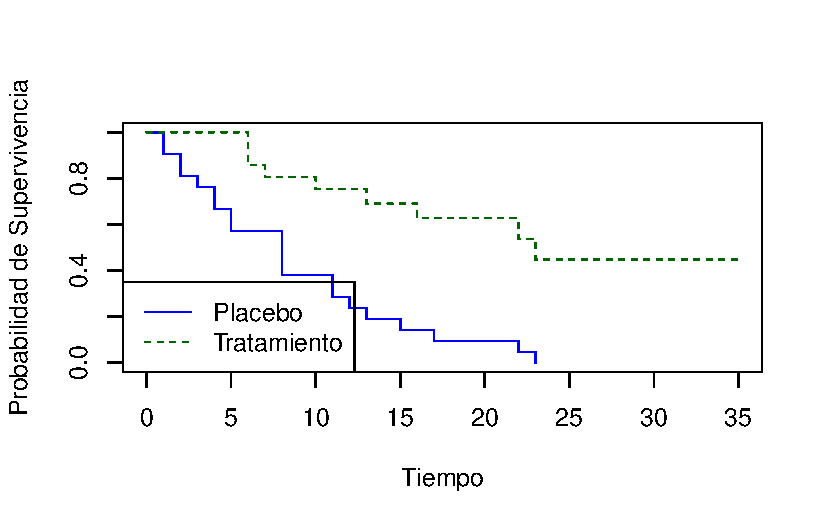
\includegraphics[keepaspectratio]{Unidad3_files/figure-pdf/unnamed-chunk-38-1.pdf}}

\begin{center}\rule{0.5\linewidth}{0.5pt}\end{center}

\subsection{Conclusión}\label{conclusiuxf3n}

\begin{itemize}
\tightlist
\item
  La prueba de log-rank es útil para \textbf{comparar curvas de
  supervivencia} entre grupos.
\item
  Es ampliamente usada por su simplicidad y poder bajo riesgos
  proporcionales.
\end{itemize}

\begin{center}\rule{0.5\linewidth}{0.5pt}\end{center}

\subsection{Actividad práctica
guiada}\label{actividad-pruxe1ctica-guiada}

\textbf{Datos}: \texttt{lung} del paquete \texttt{survival}.

Pasos:

\begin{enumerate}
\def\labelenumi{\arabic{enumi}.}
\tightlist
\item
  Cargar datos con
  \texttt{data(cancer,\ package="survival");\ head(lung)}
\item
  Crear objeto \texttt{Surv(time,\ status)}
\item
  Estimar curvas por \texttt{sex}
\item
  Probar igualdad con log-rank
\end{enumerate}

\section{Referencias}\label{referencias}

\phantomsection\label{refs}
\begin{CSLReferences}{1}{0}
\bibitem[\citeproctext]{ref-klein2003}
Klein, J. P., \& Moeschberger, M. L. (2003). \emph{Survival analysis:
Techniques for censored and truncated data} (2nd ed.). Springer.

\end{CSLReferences}




\end{document}
